%%%%%%%%%%%%%%%%%%%%%%%%%%%%%%%%%%%%%%%%%%%%%%%%%%%%%%%%%%%%%%%%%%%%%%%%%%%%%%%%
%% Para obtener PDF, ejectuar en la shell:
%%   pdflatex memoria.tex
%% (las im�genes deben ir en PNG o JPG)

%%%%%%%%%%%%%%%%%%%%%%%%%%%%%%%%%%%%%%%%%%%%%%%%%%%%%%%%%%%%%%%%%%%%%%%%%%%%%%%%

\documentclass[a4paper, 12pt]{book}
%\usepackage[T1]{fontenc}
\usepackage[utf8]{inputenc}

\usepackage[a4paper, left=2.5cm, right=2.5cm, top=3cm, bottom=3cm]{geometry}
\usepackage{times}

\usepackage[spanish]{babel}
\usepackage{url}
\usepackage{amsmath}
\usepackage{amsfonts}
\usepackage{amssymb}
\usepackage{comment}
\usepackage{color}
\usepackage{algorithm}
\usepackage{algorithmicx}
\usepackage{algpseudocode}
\usepackage{verbatim}
\usepackage{ulem}
\usepackage{caption}
%\usepackage[dvips]{hyperref}
\usepackage{pdfpages}
\usepackage{graphicx} % gr?ficos
\usepackage{subfigure} % subgr?ficos

\usepackage{enumerate}
\usepackage{listings}
%\usepackage[dvipdfm]{graphicx}

\usepackage{float}  %% H para posicionar figuras
\usepackage[nottoc, notlot, notlof, notindex]{tocbibind} %% Opciones de �ndice
\usepackage{latexsym}  %% Logo LaTeX

\title{MiStuRe: MINADO DE REPOSITORIOS DE ESTUDIANTES ORIENTADO AL ANÁLISIS DEL APRENDIZAJE.}
\author{Carlos González Sesmero}

\renewcommand{\baselinestretch}{1.5}  %% Interlineado

\begin{document}

\renewcommand{\refname}{Bibliografía}  %% Renombrando
\renewcommand{\appendixname}{Apéndice}

%%%%%%%%%%%%%%%%%%%%%%%%%%%%%%%%%%%%%%%%%%%%%%%%%%%%%%%%%%%%%%%%%%%%%%%%%%%%%%%%
% PORTADA

\begin{titlepage}
\begin{center}
\begin{tabular}[c]{c c}
%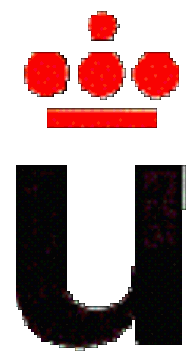
\includegraphics[bb=0 0 194 352, scale=0.25]{logo} &

\includegraphics[scale=1]{img/logo2.png} &
\begin{tabular}[b]{l}
\Huge
%\textsf{Universidad} \\
\Huge
%\textsf{Rey Juan Carlos} \\
\end{tabular}
\\
\end{tabular}

\vspace{1.5cm}

\Large
ESCUELA TÉCNICA SUPERIOR DE INGENIERÍA\\ DE TELECOMUNICACIÓN

\vspace{1.5cm}

\Large
INGENIERÍA DE TELECOMUNICACIÓN - \\ INGENIERÍA TÉCNICA EN INFORMÁTICA DE SISTEMAS

\vspace{2cm}



\textbf{PROYECTO FIN DE CARRERA}

\vspace{2.5cm}

\LARGE
MiStuRe: Minado de repositorios de estudiantes orientado al análisis del aprendizaje.

\vspace{2cm}

\large
Autor : Carlos González Sesmero \\
Tutor : Dr. Gregorio Robles

\vspace{1cm}

\large
Curso Académico 2016/2017

\end{center}
\end{titlepage}

\newpage
\mbox{}
\thispagestyle{empty} % para que no se numere esta pagina


%%%%%%%%%%%%%%%%%%%%%%%%%%%%%%%%%%%%%%%%%%%%%%%%%%%%%%%%%%%%%%%%%%%%%%%%%%%%%%%%
\pagenumbering{Roman} % para comenzar la numeracion de paginas en numeros romanos

%%%% Dedicatoria

\chapter*{}
\pagenumbering{Roman} % para comenzar la numeracion de paginas en numeros romanos
\begin{flushright}
\textit{“[...] nada está perdido si se\\
tiene el valor de proclamar\\
que todo está perdido y hay\\
que empezar de nuevo [...]”.
\\
		Julio Cortázar.}
\end{flushright}

%%%%%%%%%%%%%%%%%%%%%%%%%%%%%%%%%%%%%%%%%%%%%%%%%%%%%%%%%%%%%%%%%%%%%%%%%%%%%%%%
%%%% Agradecimientos

\chapter*{Agradecimientos}
%\addcontentsline{toc}{chapter}{Agradecimientos} % si queremos que aparezca en el índice
\markboth{AGRADECIMIENTOS}{AGRADECIMIENTOS} % encabezado 

Como Milennial educado a golpe de Hispano Olivetti y refrán castellano, un servidor tiene grabado que es de bien nacido ser agradecido, y con cariño y sarcasmo, reparte unos cuantos:\\


Empiezo por un fuerte agradecimiento a mi madre, y recordar aquello de “madre, no hay más que una”; y menos mal que una y no tres, ¿se imaginan?\\


También un gran agradecimiento a Itziar, que aunque da algo de trabajillo – ¡fuu! -, ha sido un excepcional apoyo y compañía en estos especialmente complicados últimos años.\\


Otro agradecimiento a Marcos que durante mi tránsito universitario pasó de llamar la atención a todas horas a ser un hombrecillo de provecho que tenía sus propios proyectos y dejaba a los demás hacer los suyos.\\


Un agradecimiento a toda aquella familia, amistades y allegados que durante largas temporadas de estos años compaginando mis diferentes ocupaciones solo han podido disfrutar de una pequeña parte de mí, y a la vez se alegrarán de está culminación.\\


Por otra parte un agradecimiento a la paciencia de Gregorio.\\


No olvidar al sufrido y olvidado contribuyente español, cuya indirecta contribución ha sido condición necesaria que no suficiente para que este documento haya llegado a ser redactado.




%%%%%%%%%%%%%%%%%%%%%%%%%%%%%%%%%%%%%%%%%%%%%%%%%%%%%%%%%%%%%%%%%%%%%%%%%%%%%%%%
%%%% Resumen

\chapter*{Resumen}
%\addcontentsline{toc}{chapter}{Resumen} % si queremos que aparezca en el índice
\markboth{RESUMEN}{RESUMEN} % encabezado

En el contexto actual de las enseñanzas de Grado, con un profesorado con una doble exigencia, o con la autoexigencia de proporcionar una docencia con una metodología de evaluación continua y de forma muy dinámica a la vez del requerimiento de una intensa actividad investigadora. Se intuye como más que probable, que cualquier mejora o sistema que refuerce, optimice el tiempo disponible o incremente la frecuencia y la cantidad de información realimentada con respecto a los objetivos principales de una materia, tanto como de objetivos secundarios y habilidades asociadas a ellos entre los extremos típicos del acto educativo, sea positivo para ambos.\\


Por otra parte, en el contexto descrito, en disciplinas tales como la programación donde sea posible el tratamiento automático, obtención de patrones, o mediciones de los entregables donde los alumnos demuestran su destreza y evolución. Puede ser útil la aplicación de métodos o el uso de sistemas que permitan sistematizar y extraer información valiosa con más rapidez que con la metodología tradicional. Y que permita de forma más dinámica y objetiva la transmisión y refuerzo de los conocimientos y la detección de errores o hábitos a mejorar tanto a nivel individual como a nivel grupal.\\


En este escenario, y teniendo como referencia unas experiencias previas en unas asignaturas cursadas donde se emplearon estos conceptos, se va a intentar construir una propuesta de un sistema más automatizado y generalizable, orientado a alumnos con un nivel donde todavía están por formar parte de las destrezas y hábitos de programación y materias donde se aplique la programación a pequeñas aplicaciones  orientadas al aprendizaje de otros conceptos como redes y servicios web.\\


Eminentemente, trataremos con un ecosistema donde los alumnos manejarán el lenguaje Python, caracterizado por su simplicidad y alta interoperabilidad, y la herramienta colaborativa Git como elementos comunes.



%%%%%%%%%%%%%%%%%%%%%%%%%%%%%%%%%%%%%%%%%%%%%%%%%%%%%%%%%%%%%%%%%%%%%%%%%%%%%%%%
%
%%%% Resumen en inglés

\chapter*{Summary}
%\addcontentsline{toc}{chapter}{Summary} % si queremos que aparezca en el índice
\markboth{SUMMARY}{SUMMARY} % encabezado

This Final Project, named MiStuRe, being inspired by past educational experiences, develops an automatic tool both for the programming exercises correction as for the generation of simple exams.\\


The goal of MiSture concerned to professor, is decrease the time spend about corrections and give him a lot of new information about programming capabilities and subject's knowledgement among students to improve the academic progress of class.\\


Also, the purpose is that students gain a faster and richer feedback than handmaked correction about their delivered tasks, and maybe obtain plus motivation about the subject or in order to be better.\\

%%%%%%%%%%%%%%%%%%%%%%%%%%%%%%%%%%%%%%%%%%%%%%%%%%%%%%%%%%%%%%%%%%%%%%%%%%%%%%%% 
\pagenumbering{arabic} % para empezar la numeración de página con números
%%%% Índices

%%%% Índice de contenidos
\tableofcontents 
%%%% Índice de figuras
\cleardoublepage
%\addcontentsline{toc}{chapter}{Lista de figuras} % para que aparezca en el indice de contenidos
\listoffigures % indice de figuras
%%%% Índice de tablas
%\cleardoublepage
%\addcontentsline{toc}{chapter}{Lista de tablas} % para que aparezca en el indice de contenidos
%\listoftables % indice de tablas


%%%%%%%%%%%%%%%%%%%%%%%%%%%%%%%%%%%%%%%%%%%%%%%%%%%%%%%%%%%%%%%%%%%%%%%%%%%%%%%%
%%%%%%%%%%%%%%%%%%%%%%%%%%%%%%%%%%%%%%%%%%%%%%%%%%%%%%%%%%%%%%%%%%%%%%%%%%%%%%%%
\cleardoublepage

\chapter{Introducción}
%\addcontentsline{toc}{chapter}{Summary} % si queremos que aparezca en el índice
\label{sec:intro}

En este capítulo inicial, vamos a proceder con la presentación del Proyecto de fin de Carrera que hemos denominado “MiStuRe: MINADO DE REPOSITORIOS DE ESTUDIANTES ORIENTADO AL ANÁLISIS DEL APRENDIZAJE”.\\


Con posteridad a la presentación, desentrañaremos la motivación personal con la que se empezó este proyecto, y describiremos la estructura de este documento, de modo que el lector tenga un mapa general de aquello que se va a encontrar a continuación, y adecue su lectura según su interés.


\newpage

\section{Presentación}

MiStuRe es, en primer lugar un acrónimo de MIning STUdent REpositories, que guarda semejanza gráfica o sonora con los términos español mistura e inglés mixture.\\


Misture representa a un proyecto de módulos desarrollados en el lenguaje Python en su versión 3, que intenta sintetizar una estructura que proporcione un modelo de datos, una interfaz o interfaces, y unos módulos fácilmente extensibles que permitan la automatización de la corrección de prácticas de programación y que recojan con la mayor riqueza posible la información para facilitar que el alumno tenga reportes frecuentes e instruyentes acerca de su desempeño y progresión, además de poder utilizarse sistemáticamente para reportes o análisis posteriores.\\


La utilidad del proyecto que tiene estas aspiraciones, se engloban dentro de un ámbito educativo universitario. En el que se desea poder realizar por medio de \textit{scripting} estas tareas de forma rápida automáticamente, y facilitar el análisis que permita detectar eficazmente los errores de los alumnos, e incluso de permitir incidir en otras destrezas del alumno, como la habilidad programando en cierto lenguaje, con cierto orden, simplicidad o calidad.\\


En este análisis se considera la ejecución de pruebas sobre el código o de comprobaciones sobre los ficheros entregables, para evaluar que cumplen con la funcionalidad pedida o que demuestren que la tarea ha sido efectuada correctamente, lo que implica en general un buen aprovechamiento de la actividad por parte del alumno.\\


Asimismo,  se consideran otros análisis o comprobaciones, tales como el análisis de trazas de Wireshark, útil para el caso de la corrección de actividades relacionadas con el uso o análisis de redes, protocolos o servicios web o multimedia.\\


Otro de los análisis de interés, es el del uso de la herramienta Git, que en primera instancia se puede aprovechar para conducir al alumno a la adquisición de ciertos hábitos a la hora de manejar estas herramientas con su código fuente. Y en instancias superiores, a un posible análisis pormenorizado de los colaboradores con respecto al proyecto colaborativo.\\


\section{Motivación Personal}

Aunque la idea radical que llevó a la consecución de MiStuRe no es propia, sino parte de una propuesta del tutor. Personalmente no me resultó una propuesta no motivante, ni mucho menos extraña.\\


Durante el curso de las asignaturas de tercer y cuarto curso de Ingeniería denominadas IARO -Información Audiovisual en Redes de Ordenadores- y SAT -Servicios y Aplicaciones Telemáticas-, fuimos ``conejillos de indias'', aunque no los primeros, en cursar dichas asignaturas siguiendo una metodología no muy común en el resto de las materias.\\


Dicha metodología dejaba en cierto modo de lado la típica lección magistral de pizarra, quedando reducida en muchas fases de estas asignaturas a un ajustado en el tiempo \textit{speech} sobre la materia tratada y posterior discusión de esta y de las dudas planteadas por los alumnos gracias al trabajo previo. El resto se basaba, en el trabajo y la visualización de un pequeño dosier de materiales, referencias y ejemplos, a menudo interactivos, presentados telemáticamente en las jornadas previas a la clase correspondiente, junto con la realización de tests online sobre la propia materia a continuación de realizar nuestro trabajo con este dosier.\\


La parte que está relacionada con MiStuRe, esta radicada en la vertiente práctica de estas asignaturas. Esta consistía en la realización de pequeños ejercicios de programación, incrementales, y en la corrección semiautomatizada de estos, que a cambio nos aportaba cierta información adicional sobre nuestro desempeño programando, y que probablemente, en más de un caso, nos generó curiosidad para mejorar nuestra calidad de escritura o estilo de código, por ejemplo.\\


En resumen, que dada la experiencia propia en el lado del alumno, me resulto ciertamente interesante pasar a formar parte de ello y tratar de mejorar las herramientas para potenciar esta metodología de impartir clases teóricas y prácticas.\\


Otra motivación que me llevo a adoptar la realización de un proyecto así, fueron las múltiples posibilidades de temas a profundizar o tecnologías que usar en las que aprender o ampliar el desempeño en ellas, que podía permitir la implementación de un escenario así.\\


\section{Estructura de la memoria}

Esta memoria, relativa al proyecto de fin de carrera denominado como MiStuRe, al cuál desde este momento denominaremos como Misture o proyecto para simplificar, consta de seis capítulos, apéndices sobre las nociones de uso de Misture y la instalación de las debidas dependencias para su correcto funcionamiento, y de un apartado de bibliografía.\\


En el primer capítulo, que estamos concluyendo con este subapartado, se dedica a la introducción del proyecto Misture, la motivación del autor para llevarlo a cabo, y esta explicación de la estructura que se está realizando.\\


En un segundo capítulo, el de objetivos, se detalla el problema a resolver con el proyecto Misture, concretamente de mejorar la funcionalidad de unos \textit{scripts} piloto, cuya estructura se analizará en general, y en base a este punto de partida, definiremos los objetivos.\\


En sucesivos subapartados de este capítulo, también se detallan los objetivos perseguidos por el tutor tanto como por el autor con la realización de Misture, tanto a nivel práctico como a nivel teórico.\\


Asimismo, se detallarán los requisitos funcionales que se propusieron inicialmente para Misture, que constituyen en sí mismos otro objetivo.\\


En el capítulo tercero, denominado ``Estado del Arte'', nos centraremos en detallar aquellas tecnologías, librerías o herramientas clave, así como unas reseñas sobre los ``Mining Software Repositories''.\\


En el capítulo cuarto, se describirá el diseño y arquitectura general de Misture, de sus componentes, de que elementos y utilidades nos servimos en su implementación, la estructura de las BBDD utilizadas.\\


El penúltimo capítulo, ``Resultados'', se resume que objetivos se han intentado cumplir finalmente y en que grado se han cumplido o en que estado han quedado.\\


La cuenta de capítulos queda cerrada con el de ``Conclusiones'', donde recopilamos las ideas y resoluciones a las que hemos llegado con la elaboración de este proyecto.\\


Tras el desarrollo de la memoria, adjuntamos los apéndices con aclaraciones de uso y de las particularidades de las dependencias necesarias para la ejecución del proyecto, y la bibliografía las principales referencias utilizadas a lo largo del desarrollo de Misture.



\cleardoublepage
\chapter{Objetivos}
\label{chap:objetivos}


\section{Descripción del problema}
\label{sec:des_problema}


El problema al que se quiere dar una solución es la construcción de un sistema, que a partir de unas configuraciones de entrada, y cuya especificación sea trasladable al enunciado de las actividades prácticas de alumnos de asignaturas de programación de servicios y aplicaciones sobres redes de ordenadores, pueda proceder a su corrección requiriendo los mínimos cambios o ajustes en la implementación en dicho sistema.\\


Estas correcciones es deseable que puedan realizarse lo más desatendida y automáticamente posible, permitiendo liberar tiempo al profesor y disminuir el tiempo de respuestas, además de proporcionarles con poco retraso con respecto al día de entrega de un conjunto variado de información acerca de los resultados de sus prácticas con el objetivo de incidir positivamente en el aprendizaje tanto de los conceptos de la asignatura como de habilidades en programación.\\


Los elementos que debemos considerar en la corrección del alumno son los siguientes:\\

\begin{itemize}
\item En general, un repositorio Git, no ``bare'', en el cual el alumno ha estado trabajando y pueda observarse su evolución trabajando en la actividad, cuyo directorio de trabajo contenga los entregables predefinidos por la especificación o enunciado de la actividad.\\

\item Ficheros de código fuente: trabajando casi siempre con fuentes en Python 2 o 3.\\

\item Capturas de Wireshark: dado que estamos evaluando a alumnos que cursan asignaturas relacionadas con servicios o aplicaciones lanzadas sobre redes, es un tipo de entregable muy útil para evaluar el funcionamiento de programas cliente o servidor que se entregan.\\

\item Otros ficheros de texto o XML, cuya inclusión venga justificada por contener configuraciones o datos de entrada para los \textit{scripts}, o sean en sí mismo uno de los entregables evaluables, como por ejemplo una actividad acerca del lenguaje SMIL, que es una especificación XML.\\
\end{itemize}


En base a esos entregables, tenemos que plantearnos el sistema automatizado, que nos ayude a evaluar con el mayor grado de detalle posible que la actividad ha sido entregada completamente en los términos especificados por el enunciado y la funcionalidad se cumple, demostrando el aprovechamiento de la actividad.


\section{Punto de partida}
\label{sec:puntp_partida}


Para la realización de este sistema, no se parte de cero. Ya que fruto de las nuevas experiencias docentes introducidas por el profesor, éste desarrolló unos \textit{scripts} semiautomáticos para poder agilizar la corrección y disponer los alumnos de sus reportes antes de la siguiente sesión práctica.\\


Aunque estos \textit{scripts} todavía exigen bastante intervención manual , es una muy buena primera aproximación y permite abordar todo el proceso de corrección que de otra forma llevaría días o semanas, y sin tanta cantidad de información y resultados susceptibles de evaluar y poder incidir sobre ellos en las clases.\\

\begin{figure}[H]
   \centering
   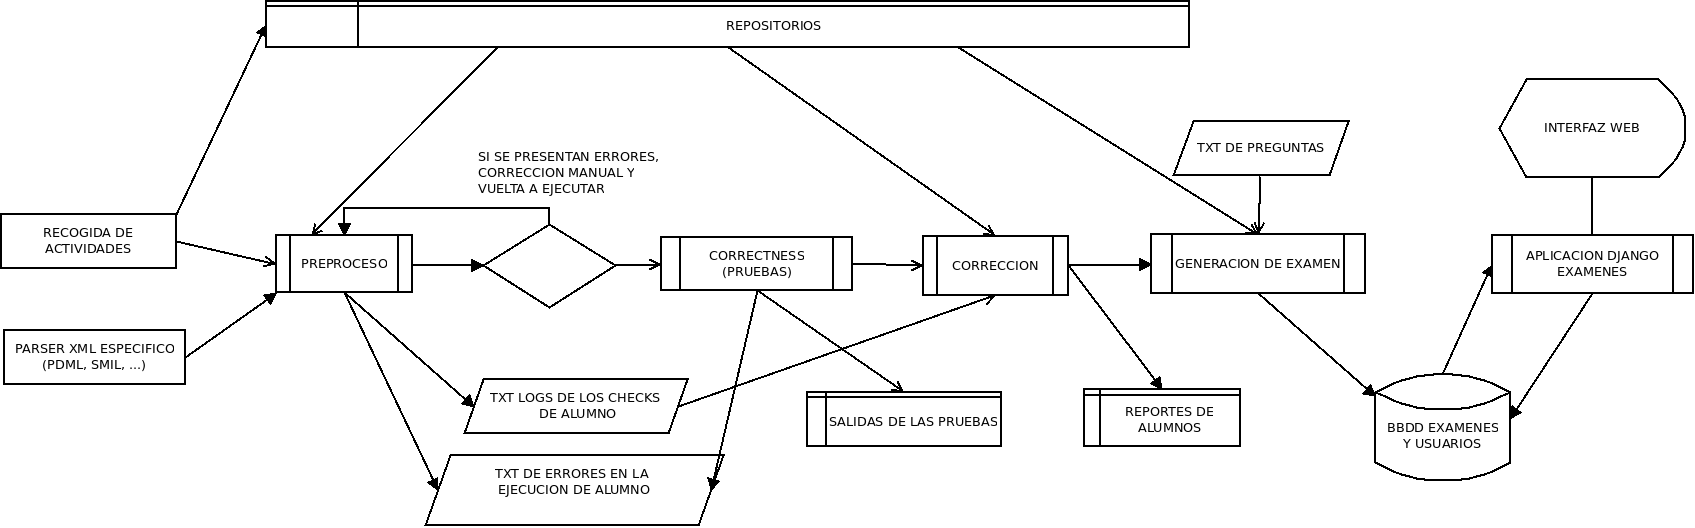
\includegraphics[width=16cm, height=7cm]{img/Diagram1_flujo_semiautomatico}
   \caption{Flujo de los scripts semiautomáticos de la experiencia piloto}
   \label{figura:flujo_semiautomatico}
\end{figure}


Según algunos reportes del profesor, con esta metodología, se podía evaluar una actividad en una mañana o una jornada, según la complejidad particular de las correcciones, y teniendo en cuenta muchos más información disponible para evaluar que otras formas de evaluación prácticas habituales en asignaturas similares.\\


Este sistema de \textit{scripts}, que se introduce en la figura anexa, se compone de los siguientes procesos, la mayoría de ellos implementados por un módulo o script Python.\\


\subsection{Recuperación de los datos}
\label{sec:rec_datos}


En general es un proceso aparte de los \textit{scripts} planteados. Cuando yo realicé estas experiencias, consistía en que los administradores de los laboratorios de la universidad automáticamente recopilaban las rutas de entrega que se habían especificado dentro del \textit{home} de cada alumno.\\


Actualmente, se solicita el usuario público de los alumnos en el servicio Github, donde se especifica que inicien un repositorio con el nombre especificado para realizar la entrega, para configurarlos en el preproceso y clonarlos.\\



\subsection{Preproceso}
\label{sec:preproceso}


En este módulo se lee y establece la configuración inicial con las especificaciones de la entrega tales como los usuarios de los alumnos, localización de repositorios, listado de ficheros a entregar, etc.\\


Una vez establecida la configuración. Se lanzan diferentes comprobaciones sobre los ficheros mediante funcionalidad python o invocando terceras utilidades con llamadas al sistema. La salida se vuelca a ficheros de texto en un formato parseable, y los errores en la ejecución de los ``checks'' a otro fichero de errores, que revisa el profesor por si tiene que tomar acciones correctoras sobre el repositorio afectado y ejecutar nuevamente los ``checks''.\\


\begin{itemize}
\item La existencia del listado de ficheros exigido.\\

\item Evaluación de errores de estilo en el código Python, con ayuda de pep8.\\

\item Evaluación de prácticas de mala calidad de código, con pylint.\\

\item Lectura del \textit{log} del repositorio Git, extrayendo el número de commits y su fecha.\\

\item En las actividades que lo exijan, ejecutar el módulo parser XML personalizado a la actividad para el chequeo de capturas Wireshark, convertidas a PDML, o la evaluación del contenido de las etiquetas y los atributos de cualquier otro fichero XML.
\end{itemize}


\subsection{Parseo XML: PDML, SMIL}
\label{sec:parseo}

La utilidad de este módulo sale a relucir en las entregas dónde los alumnos entregan capturas Wireshark con las trazas resultantes de ejecutar sus escenarios, las cuáles se convierten a PDML (ver las figuras inferiores) para facilitar su análisis. También en alguna otra actividad donde se han tratado con lenguajes XML, como el caso de SMIL.\\


\begin{figure}[H]
   \centering
   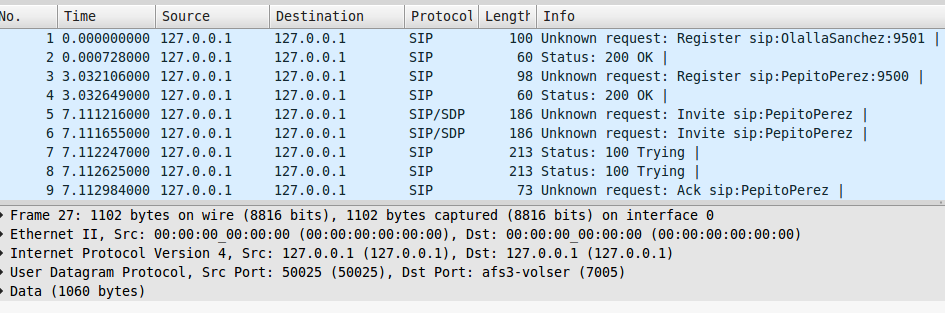
\includegraphics[width=16cm]{img/Selection_014_traza_wireshark}
   \caption{Traza de una captura de red visualizada}
   \label{figura:traza_wireshark}
\end{figure}


La aproximación que se sigue para el análisis, es utilizar el módulo SAX de Python para implementar específicamente para la actividad concreta que estamos corrigiendo, las comprobaciones sobre estos ficheros sobre las etiquetas, atributos o valores de ellas. Para demostrar que la traza o el XML ha sido generado o tiene los contenidos que se esperan, de haber realizado el alumno la tarea correctamente.\\


\begin{figure}[H]
   \centering
   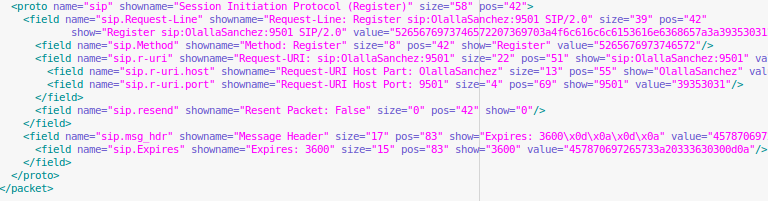
\includegraphics[width=16cm]{img/Selection_015_pdml_2}
   \caption{Extracto de un PDML de una trama SIP dentro la última capa de un paquete}
   \label{figura:extracto_pdml}
\end{figure}


Una vez el profesor ha implementado las comprobaciones en un módulo \textit{parser} específico, se invoca en el módulo de preproceso y se recogen los resultados impresos en el \textit{log} desde el módulo de corrección.


\subsection{Correctness}
\label{sec:correctness}


Correctness es el módulo de ejecución de pruebas de caja negra, se lanzan las llamadas sobre los \textit{scripts} de los alumnos para probar su funcionalidad ante determinadas entradas o ficheros de entrada, y se recogen los resultados y errores en los \textit{logs}.\\


Estas salidas se pueden comparar en el posproceso con el resultado esperado por el procesor, en el caso de actividades más sencillas o aquellas que se defina en el enunciado un formato de salida muy estricto. En caso contrario, la salida se almacena dentro del pool de ficheros de reporte del alumno para la posterior inspección del profesor.\\


\subsection{Posproceso}
\label{sec:posproceso}


La funcionalidad de este \textit{script} es parsear los logs del preproceso con el resultado de los ``checks'' y , generando un reporte en formato texto con el detalle sobre el resultado de las comprobaciones realizadas y su resultado, y el desglose de sus errores de estilo y avisos sobre líneas de código que incurren en algún uso del código no considerado de calidad según lo generalmente aceptado. Según el caso, también el resultado de las pruebas de caja negra.


\subsection{Generación de examen}
\label{sec:gen_exam}

En este script, se inyecta a una base de datos SQL, asociada también a una aplicación Django, las preguntas de la prueba que se hace a los alumnos para evaluar si el alumno conoce su propio código y cuestiones que evaluen.\\


Estas preguntas se inyectan de dos fuentes. La primera viene desde los propios ficheros fuente de la entrega, para la cual se inyecta un fragmento de ćodigo y se pregunta a cuál de los ficheros fuente pertenece.\\


La segunda fuente, es un fichero de texto, parseable, donde el profesor formula preguntas acerca de conceptos aplicados en la actividad, o cuestiones donde se le pide al alumno que indique cuál es la salida o que cambio tiene que hacer en un fragmento de código indicado.\\

\begin{figure}[H]
   \centering
   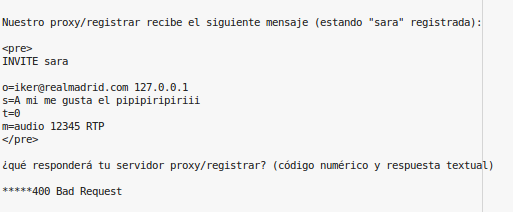
\includegraphics[width=16cm]{img/Selection_020_expregunta}
   \caption{Formato de la pregunta de examen que se sube a la BBDD}
   \label{figura:formato_examen}
\end{figure}



\subsection{Detección de plagio}
\label{sec:detec_plagio}


Esta tarea no está integrada dentro del resto de scripts, pero también forma parte del proceso de corrección, especialmente en las últimas entregas de las diferentes asignaturas.\\


En este paso del proceso de corrección, se suben las rutas con los códigos al servidor de la herramienta MOSS, donde se realiza el análisis y pasado un tiempo devuelven.\\


MOSS mide la similitud de entre ficheros texto a través de métodos estadísticos y establece esta medida fichero a fichero. Según el tipo y no es un hecho fuera de lo habitual encontrarse ante falsos positivos, especialmente si usamos MOSS para cotejar los códigos de las actividades más simples.\\

\begin{figure}[H]
   \centering
   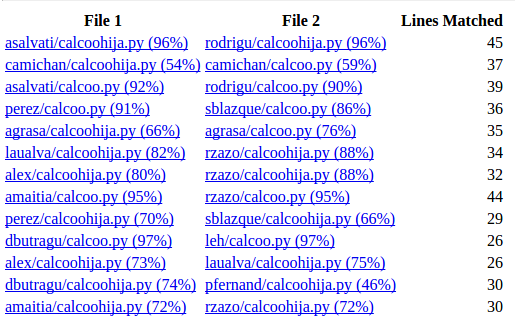
\includegraphics[width=16cm]{img/Selection_021_moss}
   \caption{Resultado que publica MOSS en una url}
   \label{figura:res_moss}
\end{figure}

\section{Requisitos}
\label{sec:requisitos}


Una vez estudiado todo el escenario de nuestro problema y la funcionalidad semiautomática de los \textit{scripts} de corrección, se estuvo definiendo de forma general entre proyectando y tutor algunos de los requisitos que se extrajeron de este análisis, obteniendo así el siguiente listado de requisitos a tener en cuenta en el sistema Misture:

\begin{itemize}
\item Análisis de qué ficheros han sido entregados en el repositorio, mejorando la experiencia del \textit{script}, limitada a verificar un listado inicial de ficheros.\\

\item Solucionar el caso frecuente de pequeñas desviaciones en los nombres de fichero.\\

\item Identificación del tipo de código de una fuente o el tipo del fichero, y algunos 	parámetros adicionales como la cantidad de líneas de código.\\

\item Análisis de la estructura de los códigos Python ampliado.\\

\item Incrementar la funcionalidad inicial que se limitaba a contar las clausulas ``class'' o ``def'' en los ficheros Python determinados inicialmente.\\

\item Análisis de errores de estilo, y calidad de código. Los pilotos cuentan la cantidad de errores de estilo de pep8 y de warnings sobre un análisis estático del código de pylint y reportan al profesor un resumen en formato texto de la cantidad de errores por tipo.\\

\item Enriquecer la funcionalidad del análisis Git, hasta ahora basado en el análisis del \textit{log} del repositorio, contando la cantidad de commits y la marca de tiempo entre primer y último commit.\\

\item Ampliar la funcionalidad del tratamiento de las capturas Wireshark, aprovechando todas las posibilidades que permite la conversión a PDML.\\

\item Como un plus, plantear, de ser posible, una utilidad de antiplagio libre como sustitutiva a MOSS.\\
\end{itemize}


\section{Objetivos generales}
\label{sec:obj_gen}


Una vez descrito el problema con el que estamos tratando, partiendo de la base de las experiencias piloto con la parte práctica de las materias, podemos establecer cuál es el objetivo.\\


El objetivo principal de Misture, es la integración de un conjunto de utilidades y de diferentes comprobaciones y pruebas de diferente índole, que van a enfrentarse contra el conjunto códigos fuentes y ficheros entregables que los alumnos generan en las diferentes actividades.\\


Esta integración debe buscar que el proceso sea lo más parecido a un flujo automatizado que reduzca el tiempo empleado por el corrector, que le permita centrarse en aquellas subtareas de una corrección donde más pueda aportar.\\


Por ejemplo, el profesor en base a estadísticas del análisis y a indagar a partir de ellos, puede detectar ciertos hábitos o malas prácticas desarrollando o aplicando los conceptos teóricos de la asignatura, o decidir dar una clase de refuerzo, enseñar cierta práctica o patrón de diseño, etc. Y esto es más valioso para todos que si tuviera que centrarse más bien en chequear entrega a entrega si un alumno ha escrito más o menos funciones, de más o menos longitud o complejidad, si su forma de escribir código es poco clara, etc.\\


Asimismo, el objetivo incluye un tratamiento más organizado de la información extraída, por ejemplo en BBDD, y la posibilidad de poder ofrecer un reporte más rico, sencillo, y fácil de ampliar o modificar frente al tratamiento que ofrecen los ficheros txt, que contienen las salidas heterogéneas de las diferentes utilidades y pruebas.\\


Para la consecución de dicho objetivo, tenemos como punto de partida el conjunto de scripts semiautomáticos que nos ha proporcionado el tutor utilizadas para las experiencias piloto, junto al reporte de incidencias u observaciones realizadas durante la ejecución y realización de alguna corrección, para intentar buscar mejoras en las funcionalidades que permitan reducir los puntos críticos en la corrección, que incapacitan la acción del \textit{script} y llevan a una revisión manual por parte del tutor. \\


\section{Objetivos Específicos}
\label{sec:obj_esp}


Aunque ya definidos los requisitos funcionales generales que exige el problema, y los objetivos generales. De estos podemos derivar algunos y concluir otros complementarios, que no debemos perder de vista para la consecución del objetivo general:\\


\begin{itemize}
\item Establecer el proyecto Python, que recogiera las funciones básicas, detectadas en las muestras de las actividades entregables de las asignaturas de programación de aplicaciones y servicios Web y multimedia en redes, adaptada a las características de las pequeñas prácticas realizadas por los alumnos.\\

\item Encontrar los mecanismos necesarios, para automatizar al máximo cada una de las funcionalidades básicas, reduciendo al mínimo la cantidad de pasos o funcionalidades semiautomáticas o manuales llevabas a cabo habitualmente por el profesor en las experiencias piloto descritas.\\

\item Como en nuestro contexto nos hallamos ante alumnos en proceso de aprendizaje de destrezas de programación. Se debe buscar el permitir cierta tolerancia en la automatización a errores por parte de los alumnos en los códigos o en los ficheros entregables.\\


Este objetivo puede en muchos casos añadir complejidad a la resolución de nuestros propósitos. Pero la detección y rectificación automatizada de estos redundaría en reducir las intervenciones manuales y re-ejecuciones de los \textit{scripts} de los diferentes pasos de la corrección.\\

\item En consecuencia a los anteriores, disminuir el tiempo dedicado por el docente en el desarrollo o adaptación del código para la corrección de nuevas actividades, su ejecución, y la recogida de resultados y reporte de los puntos críticos a revisar.\\

\item Mejora en la generación, riqueza, y comunicación del \textit{reporting} de los resultados de los diferentes análisis y correcciones que se ejecutan sobre los repositorios.\\

\item Mejorar la recogida de información extraída en las correcciones, de forma persistente y debidamente relacionada en sistemas de BBDD, permitiendo nuevos análisis posteriores, y ahorrando tiempo y re-ejecuciones en caso de errores que requieran alguna intervención manual por parte del profesor.\\

\item Interrelacionar nuestro sistema con una interfaz web, en una primera aproximación, para la realización de exámenes de verificación de autoría y conocimiento del código del alumno. Asimismo, mejorar la experiencia piloto de forma que se pueda extender la funcionalidad de la interfaz web a mostrar.\\

\item A título personal, con la realización de este proyecto, pretendía, en el momento de su elección, adquirir el conocimiento o destreza en diferentes áreas y tecnologías:\\

\begin{itemize}
\item Python 3, puesto que durante mi ciclo universitario la versión generalmente estudiada era Python 2.\\

\item MongoDB, cuyo paradigma de BBDD no había tenido la oportunidad tampoco de estudiar y practicar en ninguna asignatura.\\

\item Git, del cuál tenía un breve conocimiento básico – add, commit, pull, push – y empleado para usos individuales y no colaborativos.\\

\item Ampliar conocimientos sobre el análisis de código fuente, de repositorios, de fuentes de información heterogéneas.
\end{itemize}
\end{itemize}





\cleardoublepage
\chapter{Estado del arte}


En este capítulo se describen las tecnologías utilizadas para la realización del presente proyecto.


\section{MINING SOFTWARE REPOSITORIES}

Este Proyecto de Fin de Carrera, puede asociarse al área de los Mining Software Repositories -MSR-. El objetivo de la comunidad MSR es, aprovechar todos los datos que se generan en el proceso de desarrollo software.\\


En general, estos datos se hallan en repositorios de software, como por ejemplo repositorios de control de cambios del código fuente -como Git-, repositorios de seguimiento de bugs y errores,  o repositorios de comunicaciones, que almacenan las comunicaciones entre el equipo de desarrolladores como es el caso de las listas de distribución. Los MSR se dedican a encontrar fuentes de información provenientes de los proyectos software, estudiar sus características, encontrar técnicas para extraer de forma efectiva la información y el aprovechamiento de esos datos para mejorar los requisitos, la calidad y la trazabilidad de los proyectos, y estudiar el impacto de diferentes fenómenos en un desarrollo.\\


Gran parte del conocimiento y evolución en este campo, se presenta anualmente en la conferencia de MSR, cuya vigésimo cuarta edición se ha celebrado este año en Buenos Aires junta a la Conferencia Internacional de Ingeniería de Software.\\


En esta conferencia, se presentan los artículos sobre MSR que han sido aceptados tras su revisión y entre las actividades se encuentra la propuesta de un desafío sobre un conjunto de datos propuesto, para el cual los desafiados tienen que solucionar a través de sus herramientas o sistemas MSR y presentar un reporte de los resultados.\\


Las temáticas dentro de los MSR, entre muchas otras, podemos enumerar, por ejemplo:\\

\begin{itemize}
\item Predicción de las características del software mediante el análisis del repositorio software.\\

\item Caracterización, clasificación y predicción de defectos en el software mediante el análisis de los repositorios software.\\

\item Análisis de cambios o de nuevas tendencias.\\

\item Técnicas de visualización y modelos para los conjuntos de datos minados.\\

\item Privacidad y ética en los MSR.\\

\item Minado sobre cualquier elemento asociado a un proceso de desarrollo software. Los ya mencionados, pero también otros como licencias, \textit{logs} o las opiniones en los centros de aplicaciones y sitios de opiniones sobre los programas.
\end{itemize}


Centrándose más en la parcela relativa a este proyecto. Por otra parte, las experiencias piloto que suponen el punto de partida de este Proyecto de Fin de Carrera, fueron analizadas y expuestas en \textit{Gregorio Robles y Jesús M. González-Barahona (2013). Mining student repositories to gain learning analytics}. En éste, se expone el proceso, que ya describimos en esta memoria, y se concluye con el hecho de que proporciona importantes beneficios al facilitar la evaluación continua y realimentación frecuente a los alumnos.\\


El otro hecho que se concluye, es que un sistema de estas características, que se ha tenido que refinar en un proceso iterativo, no es posible hacerse completamente automático, y se deben tomar medidas para minimizar las tareas manuales del proceso, la principal, es que los estudiantes sigan estrictamente las instrucciones indicadas para la realización de la actividad.\\


Asimismo, a la hora de explorar formas y herramientas para explotar los datos brutos de las entregas de los alumnos, me resultó útil el análisis de las diferentes fuentes que nos podemos encontrar en un proyecto de software, que se realiza en el artículo \textit{Robles, G., González-Barahona J. M., Izquierdo-Cortazar, D. y Herraiz, I. (2009). Tools for the Study of the Usual Data Sources found in Libre Software Projects}.\\


\section{TECNOLOGÍAS UTILIZADAS} 
\label{sec:tec_use}

\subsection{PYTHON} 
\label{sec:python}


Python es un lenguaje de programación interpretado, usa tipado dinámico y es multiplataforma. Además se trata de un lenguanje de programación multiparadigma, permitiendo programación orientada a objetos, imperativa y funcional. Además posee una extensa biblioteca estándar y existen infinidad de librerías de terceros.\\


Dadas sus características, Python en muy útil como lenguaje para scripting y desarrollo rápido de aplicaciones de todo tipo.\\


Es licenciado bajo la \textit{Python Software Foundation License} desde la versión 2.1, licencia declarada libre, y compatible con GPL.\\


Fue creado por Guido van Rossum -el Benevolente Dictador Vitalicio- en los Países Bajos a finales de los años 80 y su nombre proviene de los humoristas británicos Monty Python.\\


La versión 1.0 fue lanzada en 1994, la 2.0 en Octubre de 2000 y la 3.0 fue lanzada en Diciembre de 2008. Actualmente, coexisten dos versiones de Python, la 2 y la 3, con diferencias que las hacen incompatibles, siendo las últimas versiones la 3.6.1 y la 2.7.13.\\


Python pretende ser un lenguaje fácil de leer. Para delimitar bloques se emplea la indentación en blancos en lugar de las llaves y los puntos y coma. En el mundillo Python, existe una filosofía  con unos principios de Python en cuenta a legibilidad y transparencia, recogida en el documento ``El Zen de Python'' (PEP 20). El código que siga sus principios se denomina \textit{pythonic}.


\subsection{DJANGO} 
\label{sec:django}


Django es un framework de aplicaciones web open source, escrito en Python, que aparenta seguir el patrón de diseño Modelo-Vista-Controlador. Proporciona al usuario una serie de componentes habituales en las aplicaciones web, como autenticación, sesión, administración, formularios, gestión de archivos preparados para ser usados.\\


Está orientado a realizar desarrollos rápidos, por lo que incluye un servidor web ligero para facilitar esto, aunque soporta \textit{Apache2} para la etapa de producción y servidores \textit{WSGI}. Las bases de datos soportadas son \textit{PostgreSQL}, \textit{MySQL} y \textit{SQLite3}.\\


Django fue liberado al público bajo licencia BSD en 2005, siendo desde 2008 la \textit{Django Software Foundation} quien mantiene el proyecto. La última versión es la 1.11, que será la última que soporte Python2.


\subsection{MONGODB} 
\label{sec:mongodb}


MongoDB es un sistema de base de datos NoSQL lanzado en 2009 y ampliamente adoptado por la industria. La última versión es la 3.4.4. Es orientado a documentos, los cuales se guardan en colecciones de documentos de una estructura similar a JSON -BSON-.  La equivalencia entre elementos de una BBDD SQL y NoSQL, es la siguiente:\\

\begin{itemize}
\item TABLA-COLECCIÓN\\

\item REGISTRO-DOCUMENTO

\item COLUMNA-CAMPO
\end{itemize}


Hace uso de esquemas dinámicos y no existe un esquema predefinido, pudiéndose alterar en cualquier momento, y pudiendo tener la misma colección varios documentos con distintos campos. Es recomendable en aplicaciones que necesiten almacenar datos semi-estructurados y facilitan los procesos de desarrollo iterativo.\\


No es recomendable para aplicaciones que usen intensivamente \textit{JOINS} o requieran transacciones en lugar del bloqueo a nivel de documento. Asimismo, puede presentar problemas de consistencia entre documentos, las escrituras no son verificables y puede perderse información.\\


MongoDB viene por defecto con una consola construida sobre Javascript, realizándose las consultas y operaciones en este lenguaje, y pudiéndose usar la sintaxis elemental de este lenguaje.\\


Asimismo, MongoDB tiene drivers oficiales para los principales lenguajes de programación. Para Python, el driver recomendado es PyMongo.\\


\subsection{PYMODM} 
\label{sec:pymod}

PyMODM, es un ODM sobre el driver de MongoDB PyMongo, desarrollado por ingenieros de MongoDB. Es una librería que proporciona los mecanismos para mapear la estructura de la base de datos a objetos Python, pudiéndose usar la información de la base de datos como si se tratase de un objeto.\\


\subsection{GIT} 
\label{sec:git}

Git es un sistema de control de versiones de software libre, diseñado por Linus Torvalds y lanzado en 2005. Se caracteriza por ser una herramienta distribuida, muy eficiente de proyectos grandes y que soporta muy bien el desarrollo no lineal en un proyecto, con la gestión de ramas, diferencias y mezclado de versiones.\\


En Git, los datos se modelan y almacenan como una sucesión de instantáneas de un pequeño sistema de archivos cada una, salvo el caso de ficheros idénticos entre dos instantáneas, que se referencian mediante un link. Además, todos los objetos en git son verificados mediante SHA-1 a bajo nivel, por lo que Git posee integridad.\\


Para operar con el repositorio o el historial, no es necesario  estar conectado al servidor, salvo para sincronizar los cambios, pudiendo operar todo el tiempo en local.\\


\subsection{PYGIT2} 
\label{sec:pygit2}

Librería externa de Python, que proporciona en Python la funcionalidad esencial de Git a través de \textit{libgit2}, la API en C multiplataforma.


\subsection{Pep8} 
\label{sec:pep8}

Pep8 es un ``checker'' de la guía de estilo de Python, una herramienta que valida el código Python contra las convenciones de estilo recogidas en PEP 8.\\


\section{ANÁLISIS DE CÓDIGO FUENTE} 
\label{sec:anal_cod}

El análisis del código fuente, es un tipo de análisis dentro del análisis estático de software, habitualmente realizado por herramientas automáticas, que evalúa el software sin ejecutarlo, para permitir mejorar el código, sin alterar la semántica.\\


En un análisis estático de código automático, se incluyen análisis de sintáxis del código fuente, y diferentes reglas a aplicar sobre determinadas estructuras de código.\\


En el caso del análisis humano, este se denomina comprensión de programas o también revisión de código, que es complementario al automático y permite evaluar aspectos que un sistema automático no suele cubrir, como la arquitectura, el diseño, o la forma de trabajar con elementos externos.\\


Los objetivos de estos análisis puede ser tales como la verificación de propiedades del software para seguridad o detección de código vulnerable, la mejora de la calidad del software, o mejorar el mantenimiento y desarrollo del software.\\


No obstante, el análisis de código fuente no es suficiente para evaluar o mejorar un desarrollo en todos sus aspectos, por lo que debería complementarse con otras técnicas de análisis de software, por ejemplo, los test.\\


\section{UTILIDADES DE ANÁLISIS DE CÓDIGO FUENTE EN PYTHON} 
\label{sec:utilidades_cod}


Para la realización de análisis de código en Python, nos hemos ayudado de varias herramientas, introducidas a continuación.\\


La utilidad Pep8, ya rebautizada como pycodestyle, es un ``checker'' de la guía de estilo de Python. Esta utilidad, se ejecuta sobre ficheros fuente python, y nos proporciona un listado con la localización, el código de error E*** o W*** y la descripción de los incumplimientos con respecto a la guía de PEP8.\\


Pylint, es otra utilidad de verificación de código Python bastante completa, que verifica estilo, bugs y calidad del código. También si los nombres de los elementos están bien formados con respecto a los estándares y si las interfaces declaradas son implementadas. Es una herramienta comúnmente integrada en los entornos de desarrollo y editores de código.\\


Flake8 es una utilidad que auna las comprobaciones de estilo de pep8, de errores de logica de pyflakes, y de complejidad circular. Su diseño permite la extensión mediante la inclusión de extensiones.  Por defecto incluye la extensión McCabe, que generaría errores con el codigo C9**, si detecta casos de complejidades mayores a un umbral dado.\\


Otra extensión popular es Hacking, que introduce errores con el código H***, y sus comprobaciones son las contempladas en las \textit{OpenStack Style Guidelines}, basadas en el \textit{Google Python Style Guideline}.\\

Las comprobaciones de errores de lógica de pyflakes se etiquetan mediante códigos F***. Existe una completa documentación de los códigos de error en los manuales de las diferentes utilidades.\\


\section{OTRAS HERRAMIENTAS UTILIZADAS} 
\label{sec:otras_herramientas}

El desarrollo de este proyecto se ha realizado eminentemente desde y para sistemas Linux, y concretamente se ha desarrollado y probado en distribuciones Ubuntu y Linux Mint, semejantes a los entornos que emplean profesores y alumnos en el contexto tratado.

No obstante, dado que Python es un lenguaje soportado por otros sistemas, y que en la iteración más reciente del desarrollo del proyecto se ha tendido a emplear las utilidades a través de librerías o APIs Python, o son herramientas con versión en otros sistemas. En un gran porcentaje sería portable este proyecto a otros sistemas como Windows.

En todo caso, inicialmente el desarrollo no esta considerado para otros sistemas, y exigiría la revisión de la totalidad de las dependencias de las librerías utilizadas. También sería necesaria la revisión y refactorización de algunos códigos, como por ejemplo  aquellos que emplean la librerías estándar \textit{os} y \textit{os.path}, para asegurar la plena independencia del código frente al sistema operativo.\\


Una vez circunscritos a estos sistemas, hay que recalcar que en general se ha intentado optar por el uso de editores, herramientas, librerías, DBMS de software libre, open source o en todo caso amigables con sus filosofías o licencias compatibles.\\


Aún así, durante el transcurso del proyecto, pasé a utilizar como IDE la herramienta Pycharm, que es privativa en su versión profesional, aunque contando con licencias especiales para proyectos de open source, y una versión básica con licencia no privativa.\\


En este caso, el cambio a este IDE viene justificado con una notable mejora de productividad ayudando a manejar la cantidad creciente de código, las ayudas y atajos para recordar y acceder a todas las librerías y APIs que he ido integrando, una gran ayuda en la detección de errores y \textit{warnings} previos a la ejecución, y en ejecución gracias a un potente debugger.\\


Una vez ya han sido introducidas con anterioridad las tecnologías, herramientas y librerías clave, paso a hacer una mención de dos de las herramientas que he conocido durante la realización de este proyecto, y que han sido de notable ayuda para su realización.\\

\subsection{PYCHARM}
\label{subsec:pycharm}

Como ya se ha introducido, PyCharm es un IDE multiplataforma orientado al lenguaje Python, y también al desarrollo de JavaScript y soporte para frameworks basados en estos lenguajes cono AngularJS o Django.\\


Pycharm aporta además, entre otras funcionalidades:\\

\begin{itemize}
\item Ayuda y análisis de código: autocompletado, marcado de sintaxis y errores.\\

\item Navegación avanzada entre los elementos del proyecto y del código.\\

\item Refactorización del código Python.\\

\item Depurador integrado.

\item Integración para test unitarios en Python.\\

\item Integración con sistemas de control de versiones: Git, Mercurial, Subversión, CVS.\\

\item Extensiones y disponibilidad de una numerosa biblioteca para infinidad de propósitos.\\

\item También permite la integración de herramientas externas. Por ejemplo, en nuestro caso integramos \textit{pep8} y pudiéndose chequear el estilo de cualquier módulo rápidamente.
\end{itemize}


\begin{figure}[H]
   \centering
   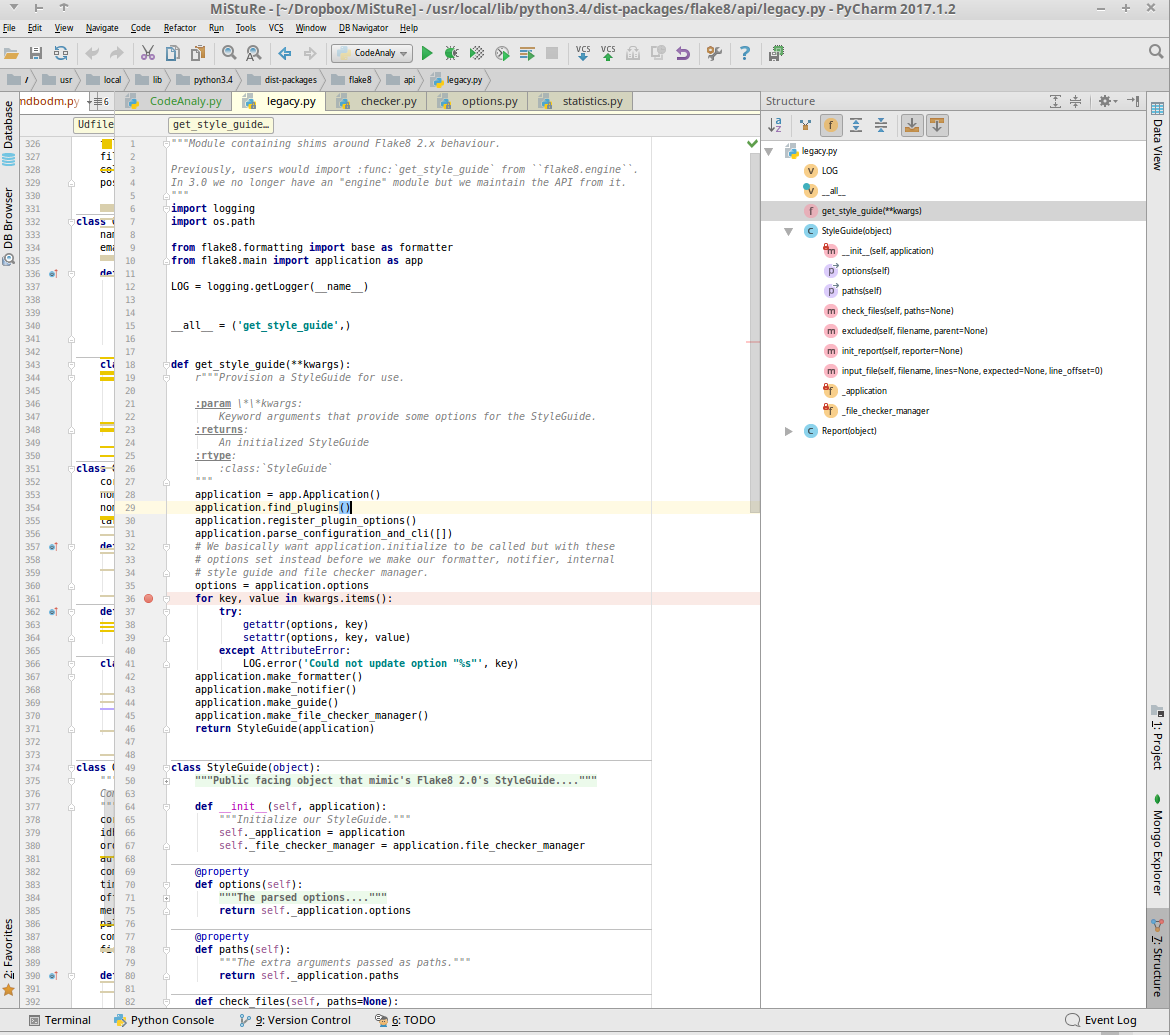
\includegraphics[width=16cm]{img/pycharm}
   \caption{Interfaz de PyCharm }
   \label{figura:pycharm}
\end{figure}



Jetbrains, la empresa desarrolladora de este producto, lo pone a disposición de los usuarios bajo un modelo que puede considerarse \textit{fremium}. Tienen disponible una versión profesional, privativa, con todas las funcionalidades y extensiones.\\


No obstante, proporcionan licencias especiales para proyectos open source no comerciales, cuyas condiciones podemos encontrar en \url{https://www.jetbrains.com/buy/opensource/}.\\


Asimismo, mantienen versiones básicas de sus productos lanzadas bajo licencias open source, como Apache 2.0, llegando a disponerse públicamente del código de algunos de ellos. Tal como es el caso de IntelliJ IDEA \url{https://github.com/JetBrains/intellij-community}, que es otro IDE desarrollado por ellos que es la propia base del IDE PyCharm.\\


En el caso de PyCharm, está versión es la denominada como ``Community Edition'', la cuál fue la que se empleo en el desarrollo y depuración de buena parte de este proyecto.\\


\subsection{ROBOMONGO}
\label{subsec:robomongo}

Robomongo es un cliente para bases de datos MongoDB con interfaz gráfica, muy ligero y de funcionalidad básica, pero suficientemente potente.\\


Además de integrar la funcionalidad del cliente shell de MongoDB, permite la escritura de scripts para mongo y la visualización rápida de las diferentes BBDD MongoDB de la conexión sobre la que se establece, asimismo de las principales características, configuraciones y contenidos de colecciones y documentos.\\


Una característica simple pero que resulta de gran ayuda, es la rapidez de navegación entre las diferentes colecciones y documentos y la posibilidad de visualización de estos en diferentes formatos como tabla, árbol, o la tradicional vista de texto en formato JSON.\\


\begin{figure}[H]
   \centering
   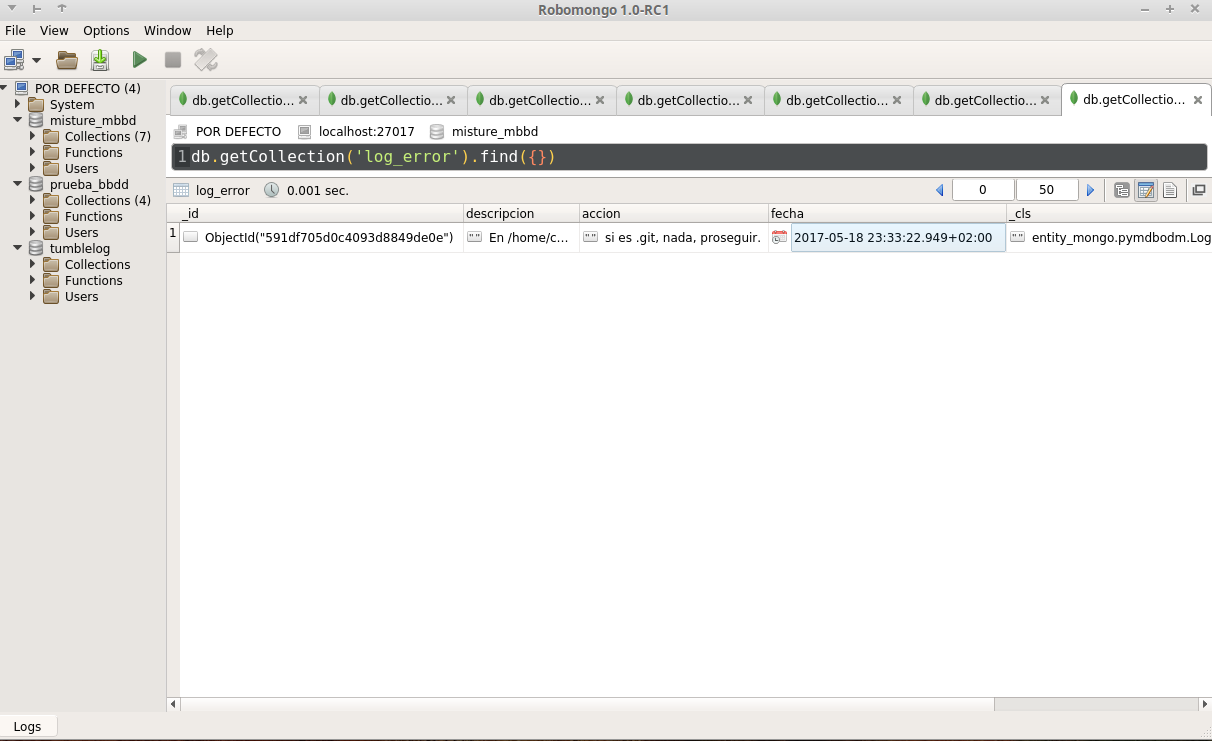
\includegraphics[width=16cm]{img/robomongo}
   \caption{Interfaz de Robomongo}
   \label{figura:robomongo}
\end{figure}


Robomongo ha estado siendo un proyecto open source cuyo código ha estado disponible públicamente. Recientemente, ha sido adquirido por la empresa Studio3T, que ha optado por mantener el proyecto en  open source \url{https://github.com/Studio3T/robomongo}, en paralelo a sus proyectos comerciales relativos a MongoDB.

\cleardoublepage
\chapter{Arquitectura y diseño.}
\label{chap:design_implement}

En este capítulo, vamos a describir la metodología de desarrollo del proyecto Misture, y el diseño y arquitectura en varios momentos de su desarrollo, respondiendo a una funcionalidad creciente y más rica.\\


Por último, se detalla de forma lo más aproximada posible la estructura de la base de datos no relacional que se emplea en el estado final del proyecto.\\


\section{Modelo de desarrollo} 
\label{subsec:modelo_desarrollo}

El desarrollo de un proyecto de software libre implica una sucesión de tareas entre el momento que se tiene una idea para resolver un problema o necesidad, y el producto u servicio final que lo satisface. Este metodología nos marca como se suceden las diferentes tareas y actividades dentro del proyecto.


Durante el desarrollo de este proyecto hemos seguido un modelo que se asemeja al modelo de desarrollo iterativo y creciente, o incremental. En este proceso creamos una primera versión del sistema que sea funcional, con el que se pueda interactuar y nos proporcione realimentación para las sucesivas iteraciones. \newpage	%TODO AJUSTE




El modelo incremental, a priori, nos proporciona las siguientes ventajas:

\begin{itemize}
\item Al desarrollar sistemas más pequeños con subconjuntos de los requerimientos o funcionalidades, reducimos el riesgo asociado a realizar el desarrollo en bloque del sistema completo.

\item Al desarrollarse progresivamente parte de las funcionalidades, se puede evaluar mejor si los requerimientos de los siguientes incrementos son correctos o hay que adaptarlos a la realidad.

\item En caso de errores o problemas, generalmente afectan a la última interacción y no a todo el conjunto, volviendo al incremento previo en el peor caso.

\item En el caso de este proyecto, permitía avanzar paso a paso en el desarrollo del sistema mientras se iba adquiriendo la experiencia necesaria para desarrollar mejor o redefinir mejor los siguientes incrementos.
\end{itemize}


Además, este modelo tiene gran similitud con el modelo que nuestro profesor adoptaba para la evolución de las prácticas de sus asignaturas durante el curso. Estas empezaban con prácticas sencillas o introductorias, a las que se le iban añadiendo elementos, funcionalidades y complejidad hasta llegar a la práctica final, que en realidad era una sucesión de incrementos a partir de una estructura inicial que se había establecido prácticas atrás.


Para observar esto último, en el caso de este proyecto, disponíamos de algunas muestras de grupos de repositorios de las actividades en diferentes etapas del trimestre los cuales, por ejemplo, podemos clasificar según a la exigencia que nos va a suponer para nuestro sistema corrector Misture. \newpage	%TODO AJUSTE




\textbf{GRUPO 1}


\begin{itemize}
\item Actividades en las semanas iniciales del trimestre o introductorias.

\item Pequeños proyectos con poca cantidad de código y elementos que exige un análisis de código Python más simple.

\item Salidas de ejecuciones más sencillas: cierto fichero con un contenido concreto, cadenas cortas de valores concretos, etc.

\item Puede requerir algunas comprobaciones sencillas sobre ficheros o documentos XML

\item Por el momento, al alumno se le está introduciendo en temas de calidad y estilo de código y es suficiente contar los errores e imprimirle al alumno qué errores comete, qué significan y en qué código se produce.
\end{itemize}

\vspace{1cm}
\textbf{GRUPO 2:}


\begin{itemize}
\item Actividades de etapas avanzadas del trimestre o de materias de mayor nivel.

\item Escenarios de mayor cantidad y complejidad de código fuente: aplicaciones cliente-servidor con lógicas complejas, desarrollo de aplicaciones sobre frameworks que conllevan mayor complejidad en la estructura del proyecto entregado, etc.

\item Análisis de código Python más complejo y rico.

\item La propia prueba de ejecución de la aplicación o aplicaciones se vuelve más difícil, y no nos sirven de igual forma cierto tipo de pruebas de ejecución en unos escenarios u otros.

\item En este punto, es interesante obtener información más rica sobre estilo y calidad de código y errores, para poder luego analizarse o reportarse asociado a su fichero fuente, u observar la evolución temporal de la calidad y errores de nuestro código.
\end{itemize}


De acuerdo al modelo de desarrollo descrito, en una fase inicial recogimos de forma general los requerimientos del sistema completo en base a la descripción del problema y las experiencias previas descritas en el Capítulo \ref{chap:objetivos} de la presente memoria.


Una vez se disponen de los requisitos, se crea una versión inicial funcional, que comenzamos con un modulo principal que dispone de las configuraciones básicas para obtener los repositorios y conocer los requisitos básicos como qué ficheros deben entregarse.


A partir de ese versión inicial, se fueron añadiendo los módulos con los diferentes grupos de funcionalidades, los cuáles íbamos probando frente a las muestras de los repositorios de alumnos. Es decir, realizábamos un incremento para agregar funcionalidad básica de análisis de código Python, posteriormente otra iteración para la extracción de información básica del repositorio Git, etc.


Entre dos incrementos, las únicas entradas de las que disponemos son los requisitos y el resultado de la interacción entre el cliente y el resultado del incremento anterior. En este caso el cliente somos nosotros probando los repositorios de las actividades de los alumnos.


Para simplificar la explicación del diseño de Misture, vamos a reducir la explicación de todo el proceso al detalle de dos estados, que vamos a denominar iteración 1 e iteración 2, que realmente componen una sucesión de incrementos que llevaron a esos dos estados del proyecto.


Esta división, asimismo, tiene también como justificación el hecho de que el estado descrito en la primera iteración es más próxima a las actividades caracterizadas del grupo 1 descrito anteriormente, y la iteración 2 recoge un estado más cercano a resolver las necesidades de las actividades descritas en el grupo 2.

\section{Iteración 1:}

Vamos a describir el diseño de los diferentes módulos que componen este primera sucesión de incrementos. En la figura de abajo se muestra un esquema de flujo de está primera versión de Misture.


En este diseño, para el almacenamiento y tratamiento de todos los datos extraídos en los diferentes análisis, se emplearon ficheros en las transacciones con las utilidades externas y para generar logs de errores e imprimir el reporte final ordenado. También se utilizaron estructuras dinámicas como listas, diccionarios y una jerarquía de clases Python que modelaban los diferentes objetos y las relaciones entre ellos que identificábamos en este escenario, tales como actividad, alumnos, repositorios, ficheros, elementos de código, estadística, error de estilo, etc.


Esta jerarquía de clases, es una primera versión del modelo de datos que será usado en la iteración 2 y que se detallará posteriormente en el apartado DISEÑO DE BBDD.



\begin{figure}[H]
   \centering
   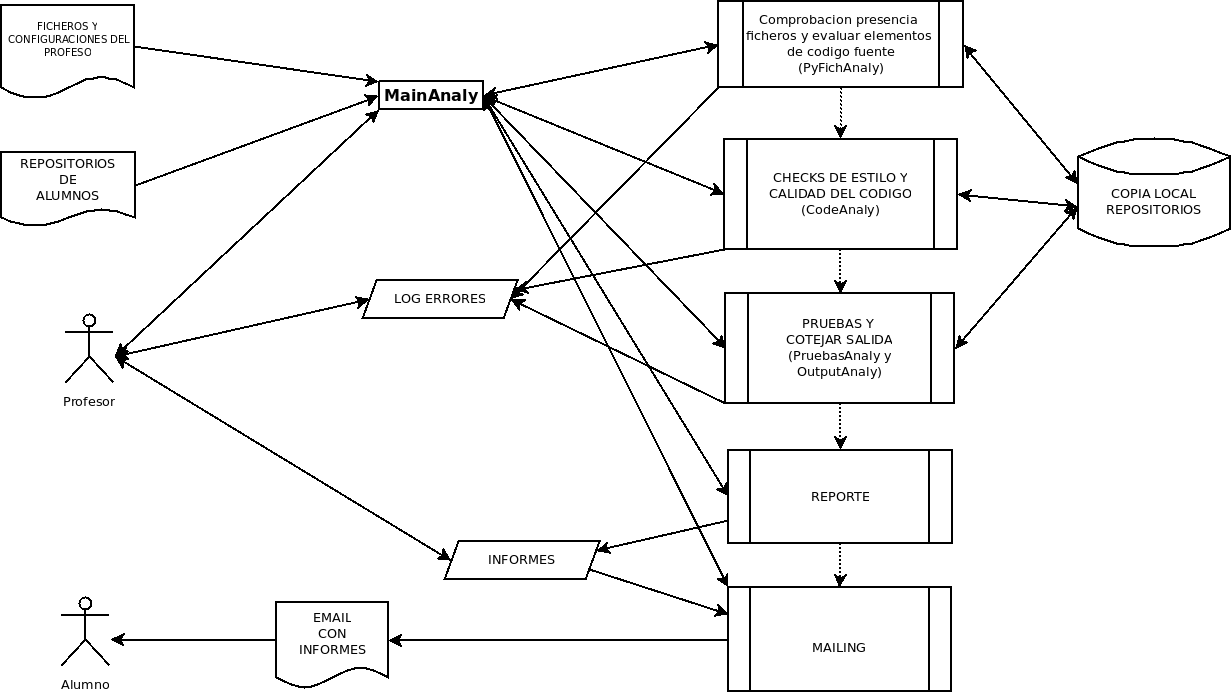
\includegraphics[width=12cm]{img/Diagram2_iteracion1}
   \caption{Flujo de la iteración 1.}
   \label{figura:ite1}
\end{figure}


\subsection{Módulo principal}

En el modulo \textit{MainAnaly}, se establece la configuración básica de la actividad a corregir, como la ubicación de los repositorios asociados a los logines de alumnos, los nombres de los ficheros y códigos fuentes que deben estar en el repositorio. Así como las tuplas con las llamadas a los programas del alumno, y las salidas que debe obtener el programa en caso de funcionar correctamente según la especificación de la actividad.


Este módulo, también se encarga de cargar esta configuración en la jerarquía de clases del escenario, inicializar los logs para la actividad, y establecer una ubicación para los reportes individualizados.


A continuación, se realiza las diferentes llamadas a los módulos de análisis, a los que se les proporciona como parámetros los objetos adecuados del escenario -repositorio, fichero, etc- y se recoge los resultados del análisis, asociándolos al objeto del mundo Misture correspondiente.

Al final del flujo se invoca a los objetos Misture para que se vuelque su información ordenada a los ficheros de reporte del alumno asociado, y se ordena al módulo de comunicación enviar en lote todos los reportes a los alumnos.

\subsection{Módulo de análisis de código Python}

Este módulo, llamado \textit{PyfichAnaly}, implementa la funcionalidad relativa a la identificación de los ficheros presentes en el repositorio del proyecto, en función de una lista definida de ficheros que se esperan de los alumnos.


Como novedad, en este análisis se detecta si al alumno le falta alguno de los ficheros requeridos por la práctica, y a través de una pequeña heurística intenta deducir si hay otros ficheros que de nombre similar que puedan serlo.


Esta heurística, se basa en el algoritmo de Levenhstein. Este algoritmo tiene la capacidad de medir la cantidad de operaciones de inserción, borrado o cambio de caracteres que hay entre dos cadenas de texto.


Por tanto, en caso de que se encuentren archivos huérfanos en la lista de ficheros requeridos y en el repositorio, y siempre que no supere un umbral, se entiende que el fichero con la menor distancia de Levenhstein es aquel que nos falta, y por tanto, se renombra y se prosiguen los análisis.


Una vez identificados los ficheros disponibles, se identifican los que son ficheros fuente Python, y se llama a la clase \textit{PyModuleCont}, que analiza el código fuente del fichero a través de patrones regulares y funciones de las librería \textit{re} de Python, cuya muestra se adjunta en la figura inferior.


De dicho análisis, asociamos al fichero Python los elementos clase, método y función que contengan, junto a su nombres.


\begin{figure}[H]
   \centering
   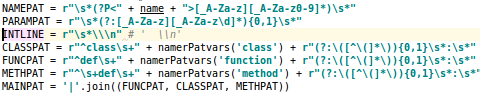
\includegraphics[width=16cm]{img/Selection_022_pyanaly_regex}
   \caption{Patrones utilizados para identificar elementos de código y su nombre}
   \label{figura:regex}
\end{figure}

\subsection{Módulo de análisis de calidad de código}

En el módulo \textit{CodeAnaly}, se implementa la funcionalidad de análisis de calidad del código, que en esta iteración del desarrollo de Misture, se realiza con ayuda de las utilidades \textit{Pep8}, para el análisis de estilo, y \textit{Pylint}, para el análisis estático del código.


El procedimiento de análisis de estilo, se implementa en la clase \textit{Pep8Analy}, es una clase con los atributos necesarios para almacenar los errores de estilo, ficheros en que se producen, y estadísticas de los errores.


\textit{Pep8Analy}  recibe como configuración las rutas de los ficheros Python a analizar, y los códigos de error que no deben ser tenidos en cuenta para este análisis. Y se inicializa invocando a la utilidad \textit{Pep8} como se indica abajo, para recopilar los errores detectados y un sumario de estadísticas.

\begin{center}
\begin{verbatim}
$ pep8 --repeat --show-source –ignore=<cods_error> <rutas_py>
$ pep8 -q --statistics <rutas_py>
\end{verbatim}
\end{center}


Por otra parte, también se implementa una clase \textit{PylintAnaly}, que con un funcionamiento semejante al de \textit{Pep8Analy}, extrae y guarda de forma estructurada los errores \textit{Pylint} y la nota de calidad del código obtenidas de la utilidad llamada de la siguiente manera.

\begin{center}
\begin{verbatim}
$ pylint --disable=<codigos_error> <ruta_py1 ruta_py2 ...>
\end{verbatim}
\end{center}


\subsection{Módulo de pruebas de ejecución}

A través del módulo \textit{PruebasAnaly}, en esta versión de Misture se ejecutan y almacenan los resultados para ser asociados a la corrección del alumno, una batería de pruebas que debe ser proporcionada al ser invocado la interfaz del test, implementado en la clase \textit{testPr} del módulo.

Cada elemento de la batería de pruebas es una prueba simple a través de una llamada a uno de los programas o scripts del alumno, sobre la ruta de su repositorio. Cada prueba, esta representada por una 3-tupla de etiqueta, prueba a ejecutar, y un tercer elemento que es una tupla con el contenido de las líneas que debemos recoger a la salida estándar de la prueba para dar por válida la prueba.


\begin{figure}[H]
   \centering
   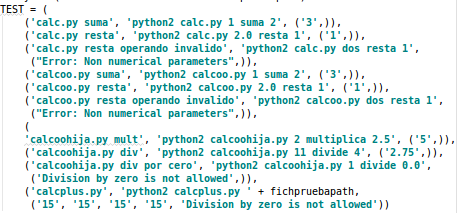
\includegraphics[width=16cm]{img/Selection_024_testcodigo}
   \caption{Tuplas con la batería de pruebas}
   \label{figura:testcodigo}
\end{figure}

La clase \textit{testPr} itera sobre cada una de las tuplas de prueba, ejecuta la prueba, e invoca a un pequeño módulo denominado \textit{OutputAnaly}, que chequea a través de funciones de texto y de la librería \textit{re} de Python que la salida recogida es compatible con la salida esperada, permitiendo cierta incertidumbre introducida por cambios en la capitalización, introducción de separadores o caracteres blancos, etc.

\subsection{Módulo de análisis de GIT}


En esta versión de Misture, se implementa un análisis sencillo de repositorio Git. Dicho análisis, se realiza a través del parseo de la salida de la siguiente llamada a Git.
\begin{center}
\begin{verbatim}
$ git log <ruta_repo_alumno>
\end{verbatim}
\end{center}

A la salida del \textit{log}, se le extraen mediante funciones de la librería \textit{re} de Python y los patrones adecuados los datos del autor del \textit{commit}.


Asimismo, podemos proporcionarle un listado de palabras o raíces de palabras que consideramos clave en los \textit{commits} de la actividad que corregimos por su significancia, obteniendo  del análisis el número de apariciones, y en consecuencia, una medida sobre si el alumno etiqueta los \textit{commits} con buen criterio.

\newpage	%TODO AJUSTE

\begin{figure}[H]
   \centering
   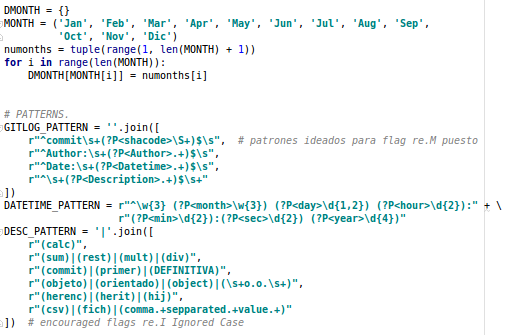
\includegraphics[width=16cm]{img/Selection_025_gitlog_patterns}
   \caption{Regex utilizados para el análisis del log}
   \label{figura:reg_analisis_log}
\end{figure}

\subsection{Módulo de comunicación}

Con el objetivo de dotar de nuevas funcionalidades a Misture y automatizando y reduciendo el tiempo necesario para todas las tareas. Se implementó una funcionalidad con el objetivo de poder comunicar masivamente el resultado de las prácticas. Esta funcionalidad la implementamos en el módulo \textit{mailing}.

En dicho módulo, a través la funcionalidad de las librerías \textit{smtplib} y \textit{email} de Python, o la API del servicio de emailing \textit{SendGrid}, hay implementaciones para realizar el envío automatizado de los reportes, siempre y cuando se proporcionen las credenciales de acceso.	\newpage %TODO AJUSTE

\section{Iteración 2:} 
\label{subsec:iteracion2}

Una vez descrito el diseño y funcionalidad de Misture en el estado anterior, podemos observar que el diseño propuesto en ese punto, introduce algunas pequeñas mejoras en cuanto a funcionalidades, organización y modularidad del sistema, especializando las tareas y diferentes tipos de análisis .


Asimismo, se ha establecido un universo de objetos que modela aproximadamente los elementos que nos vamos encontrando en una corrección automática y la generación de resultados de \textit{checks}, y así disponer de toda la información extraída en los análisis de una forma estructurada.


De esta forma, se facilita la recuperación de la información, pudiéndose elaborar diferentes informes al final del proceso corrección partiendo de la misma estructura de información, en lugar de componer una combinación heterogénea y por separado para alumno y profesor de trazas de diferentes ficheros sobre la marcha. También se facilita la posibilidad de añadir con más facilidad en pasos posteriores del proceso, otros análisis a partir de la información estructurada de la corrección. Por ejemplo, para añadir un pequeño análisis de la actividad a nivel de grupo, mediante la agregación de la información sobre cualquiera de los análisis.


Aun así, a pesar del trabajo desempeñado, la funcionalidad no supone una mejora cualitativa con respecto al sistema de \textit{scritps} de preproceso y corrección que se plantea en las experiencias piloto de los que partimos. Además, seguimos circunscritos a la corrección de entregas de tamaño reducido, con un pull de ficheros cerrado, y comprobaciones basadas en el parseo de la salida de trazas de terceras utilidades.


Por tanto, esta aproximación, una vez nos planteamos ampliar la funcionalidad, añadir más información para cada uno de los análisis, y trasladarlo a las correcciones de entregas más complejas y avanzadas, nos damos cuenta que es algo limitada para tales intenciones.


Tras recapitular estas ideas, es posible vislumbrar qué líneas vamos a seguir en la mejora del proceso. Por tanto, en los sucesivos incrementos de funcionalidades, se buscaron las siguientes mejoras:

\begin{itemize}
\item Estructurar la información en BBDD

\item Especializar aún más los módulos de análisis.

\item Búsqueda de APIs Python de las utilidades que se emplean para el análisis, o de alternativas que nos ayuden a tal fin.
\end{itemize}

A raíz de los cambios introducidos en el diseño de los sucesivos incrementos que realizamos en esta segunda versión de Misture, la estructura del código resultante se amplió, constando el proyecto con la siguiente estructura:

\begin{itemize}
\item El \textit{script} o módulo principal, desde el que se deben especificar las configuraciones y entradas -listados, ruta de ficheros del profesor, etc- necesarias para la corrección, y se invocan las llamadas a los análisis disponibles con los parámetros que el profesor quiera lanzar.

\item Un paquete de entidades –denominado \textit{entities}- donde se representan a los objetos del universo Misture, mapeados como documentos a una BBDD MongoDB.

\item Un paquete que contiene todos los módulos especializados que proporcionan acceso a cada pequeña funcionalidad de análisis implementada a través de, denominado \textit{Analyx}.

\item Se añade un paquete, cuya función consiste en hacer de intermediario entre los tres elementos anteriores, denominado \textit{funcionalityx}. Proporciona al módulo principal la interfaz sobre las funcionalidades de análisis a usar. Después, para cada funcionalidad, se encarga de invocar las operaciones y análisis especializados necesarios de los módulos del paquete \textit{analyx}. Y por último, es el encargado de interaccionar con las entidades del paquete \textit{entities}, de forma que la información que recibe de los análisis la almacene estructurada en los objetos del ODM, que se almacenaran de forma persistente en la BBDD.
\end{itemize}

A continuación, se describen dichos paquetes.

\begin{figure}[H]
   \centering
   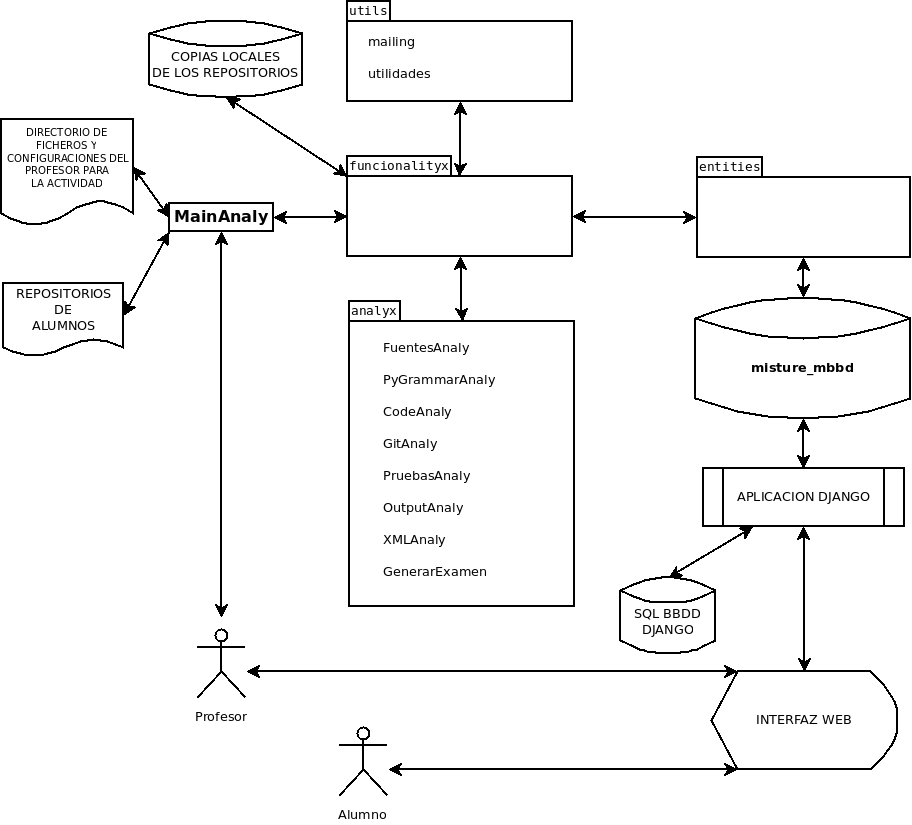
\includegraphics[width=16cm]{img/Diagram3_iteracion2}
   \caption{Relación entre los paquetes y elementos en esta versión de Misture}
   \label{figura:regex}
\end{figure}



\subsection{Módulo principal} 
\label{subsec:mod_principal}

Durante el transcurso de las iteraciones, se sigue manteniendo en el diseño el módulo principal como elemento de interacción con el profesor para la configuración, control y uso de la funcionalidad de Misture. La idea es que este módulo abstraiga el resto del sistema Misture y únicamente pueda usarse con la interfaz que proporcionemos a través del paquete \textit{funcionalityx}, siendo sólo necesario editar la configuración y llamadas a los análisis deseados para realizar cualquier corrección.


Se mantiene la necesidad de disponer de los listados de alumnos y de la ubicación o url de los repositorios, así como de las tuplas con las pruebas de caja negra a ejecutar. Además, se introduce como novedad la definición en la configuración de un directorio del profesor especifico para cada corrección, donde se depositan los ficheros externos necesarios para las funcionalidades como las preguntas de examen, ficheros de entrada u otros módulos, por ejemplo la implementación de un cliente o servidor para usarlo en las pruebas contra la implementación de los alumnos.

\subsection{Paquete de entidades} 
\label{subsec:paq_entities}

En la primera versión de Misture, se implementó una pequeña jerarquía de clases, con relaciones entre sí, que modelaban las diferentes realidades dentro de la corrección, con sus datos y relaciones entre ellos: una actividad, una corrección de actividad sobre un repositorio, un error de estilo o código, etc.


El siguiente paso en el diseño, ha sido trasladar este modelado a BBDD, de forma que podamos almacenar y recuperar sistemáticamente la información, y disponer de toda la información para posteriores reportes o análisis.


Al establecer el diseño de este paso, se optó por una base de datos no relacional como MongoDB, ya que para nuestro desarrollo incremental era más ágil y menos problemático no tener la exigencia de cumplir con un esquema fijo en los datos en todo momento.


Por otra parte, para poder centrarnos en la lógica de negocio de Misture, y abstraernos lo máximo posible de los accesos a datos, optamos también por el uso de un ODM, eligiendo \textit{PyMODM}. De esta forma, podemos mantener la lógica de nuestro universo de objetos Misture y ampliarla con mayor facilidad.


Asimismo, \textit{PyMODM} nos permite establecer el tipo de sus campos y otras restricciones, además de implementar validaciones como vemos en las figuras. Estas siempre se realizan a nivel de aplicación y no en BBDD.


\begin{figure}[H]
   \centering
   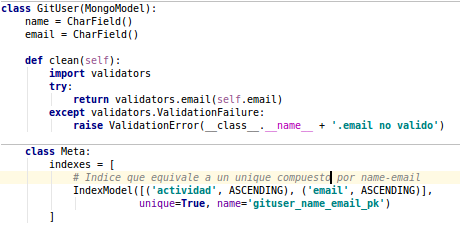
\includegraphics[width=16cm]{img/Selection_026_mongomodel}
   \caption{Un objeto Misture como documentos de una colección en MongoDB vía ODM}
   \label{figura:iter2}
\end{figure}

\begin{figure}[H]
   \centering
   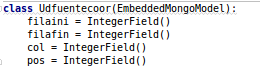
\includegraphics[width=8cm]{img/Selection_027_mongoembdoc}
   \caption{Representación de un documento sin colección, embebido en otro documento}
   \label{figura:mon_emb}
\end{figure}


\subsection{Paquete de funcionalidades} 
\label{subsec:paq_functs}

Como ya se ha introducido, este paquete \textit{funtionalityx} se encarga de implementar las funcionalidades de Misture a alto nivel, delegando las diferentes tareas que conforman un análisis a los módulos especializados del paquete \textit{analyx}, estructurando los datos recibidos en los objetos del ODM para su guardado en las colecciones de MongoDB, y atendiendo a las llamadas que recibe de la interfaz que sirve al módulo principal.


Las funcionalidades que podemos invocar, son las que se detallan a continuación.

\begin{itemize}
\item Análisis de ficheros del repositorio.

\item Análisis de elementos del código Python.

\item Análisis de estilo y calidad del código.

\item Análisis de repositorio Git.

\item Análisis de XML y trazas de Wireshark.

\item Generación de examen.
\end{itemize}


\subsection{Paquete de análisis} 
\label{subsec:paq_anals}


En el diseño de las siguientes iteraciones de desarrollo, se mejoraron y ampliaron las funcionalidades de los análisis, buscando obtener funcionalidades a partir de librerías Python para Git, Pep8, u otras alternativas, lo que nos facilitaba el acceso a más opciones y datos.


Esto, junto con el resto de cambios comentados, justificó la reestructuración del proyecto, volcando dentro de un paquete los módulos de los diferentes análisis, aunando las viejas y nuevas funcionalidades implementadas.

A continuación los enumeramos.


\subsubsection{Módulo de análisis de ficheros entregados} 
\label{subsec:mod_anal_fich}

Con el objetivo de ampliar el análisis del contenido de la entrega, se crea un nuevo módulo, \textit{FuentesAnaly}, que analiza el árbol del proyecto entregado, sin limitarse a evaluar un listado cerrado de ficheros, funcionalidad que mantiene el modulo \textit{PyFichAnaly}.


En este módulo, se lee todo el árbol del directorio, almacenándose para su posterior guardado estructurado en la BBDD.


Asimismo, nos servimos de la herramienta \textit{Sloccount}, ejecutado sobre el directorio del repositorio del alumno, para obtener parámetros de lenguaje, cantidad de líneas de código, de los ficheros fuente que se detecten. Con esos datos junto a la extensión del fichero, le asociamos el tipo de fichero.

\begin{center}
\begin{verbatim}
$ sloccount --details --follow --duplicates <path_directorio>
\end{verbatim}
\end{center}


Todos estos datos, se guardaran debidamente relacionados en la colección \textbf{Udfile} de nuestra BBDD.


\subsubsection{Módulo de análisis de GIT} 
\label{subsec:mod_anal_git}

Para el desarrollo de una funcionalidad de análisis del repositorio Git más rica, se implementó un nuevo módulo \textit{GitAnaly}, que permite a través de la introducción de la librería de Python Pygit2 el manejo de repositorios y la lectura de la estructura y contenidos de éste.


Este módulo proporcionamos, por una parte, funcionalidad para descargar, copiar o clonar los repositorios y puedan realizarse el resto de operaciones y análisis. Por otra parte, aprovechando la API de Pygit2, implementamos funcionalidad para extraer la información de las ramas locales y remotas. También se implementa otra funcionalidad la cual nos extrae en orden topológico la sucesión entre dos commits cuyo sha-1 se índique, o entre HEAD y el primero en su defecto. Se analizan todos los datos de un \textit{commit}, disponiendo en este caso de una información más completa.


Entre esta información adicional, se extraen ciertas estadísticas para su almacenamiento:

\begin{itemize}
\item Frecuencia entre los \textit{commits}.

\item Extracción de palabras clave de un \textit{commit}: se extraen la lista de palabras clave resultante de normalizar el comentario, suprimir las palabras consideradas de un listado de irrelevantes.
\end{itemize}

\begin{figure}[H]
   \centering
   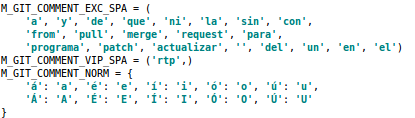
\includegraphics[width=16cm]{img/Selection_028_git_comentarios}
   \caption{Parámetros para la extracción de significantes de comentarios de \textit{commits}}
   \label{figura:git_commnet}
\end{figure}

Toda la información extraída según cada funcionalidad, se proporciona estructurada y los \textit{commits} relacionados entre sí para que pueda ser todo almacenado en BBDD.


\subsubsection{Módulo de análisis de código Python} 
\label{subsec:mod_anal_python}

En el análisis de los elementos del código fuente, introducimos en el diseño las funcionalidades que aportan la librería estándar \textit{Ast} y la librería externa \textit{Astor}, cuya función es la de procesar árboles de gramática abstracta, en Python.


Con ellas, podemos recuperar todos los elementos de código y sus propiedades en una estructura de árbol. Para la funcionalidad de este módulo, ambas librerias nos simplifican la implementación y abre nuevas posibilidades a futuras automatizaciones de Misture. \textit{Astor} nos proporciona algunas capacidades adicionales para manipular estos árboles y convertir el árbol a otras estructuras, incluyendo su impresión a texto de nodos de código.


Esta funcionalidad la añadimos al módulo \textit{PyGrammarAnaly}, para extraer datos por módulo sobre sus clases, métodos, línea y nombre, y pueda volcarse en la colección \textbf{UdFuente}. No obstante, mantenemos la anterior funcionalidad de la clase \textit{PyModuleCont} y la trasladamos a este módulo, para su uso en prácticas pequeñas o sobre versiones antiguas de Python.


\subsubsection{Módulo de análisis de estilo y calidad de código} 
\label{subsec:mod_anal_codigo}

En la implementación se mantuvo en gran medida la funcionalidad del módulo \textit{CodeAnaly}. Se sustituyeron las llamadas a las utilidades por sus librerías equivalentes en Python. Se consiguió una pequeña mejora en la extracción de la información de Pylint obteniendo la salida de los errores en JSON.


La principal novedad, es la introducción de una nueva utilidad de análisis de \textit{Flake8}, que combina, el análisis de estilo de \textit{Pep8} con el análisis estático de \textit{Pyflakes}, similar a \textit{Pylint}. Asimismo, permite la instalación de otros plugins para ampliar el análisis. Por lo que extendemos, con los paquetes \textit{McCabe} y \textit{Hackings}, aumentando la cantidad de comprobaciones y códigos de error disponibles.


\subsubsection{Módulos de análisis de XML y trazas Wireshark}
\label{subsec:mod_anal_xml_wireshark}

En el análisis de los \textit{scripts} semiautomáticos de las experiencias piloto, comentamos que existía un análisis de ficheros XML, que consistía en implementar un pequeño parser SAX específico para la corrección que comprueba la validación deseada sobre los elementos XML.


En esta versión,  se ha empezado a introducir una aproximación mediante análisis del árbol DOM, con ayuda de la librería Beautiful Soup 4, que genera dicho árbol y nos proporciona un potente conjunto de funciones para navegar.


Gracias a esto, hemos implementado un pequeño analizador dedicado a PDML que obtiene algunas estadísticas de las trazas. Como por ejemplo, para extraer la composición de tramas de los paquetes de una trama.

\begin{figure}[H]
   \centering
   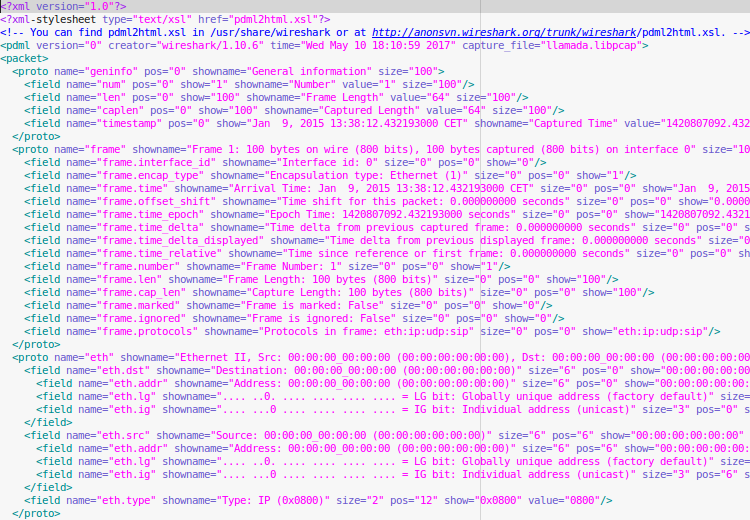
\includegraphics[width=15cm]{img/Selection_015_pdml_1}
   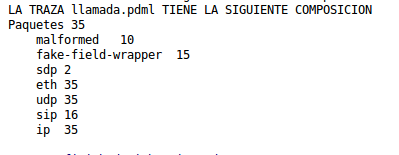
\includegraphics[width=8cm]{img/Selection_029_pdml}
   \caption{El PDML de la traza son elementos \textit{packet} con elementos \textit{proto} en su interior.}
   \label{figura:pdml}
\end{figure}


\newpage

\subsection{Generación de examen}

En el diseño, se incluye este módulo que permite la generación y carga para la corrección de cada alumno, de un conjunto de preguntas acerca del código y de los conceptos que el profesor quiera poner a prueba. Para ello, consideramos dos fuentes:

\begin{itemize}
\item Se carga un fichero JSON con las preguntas desde la ruta que se le indica como parámetro. La estructura de este JSON es una lista de objetos pregunta con los elementos enunciado, pregunta, tipo, opciones, resultados, etc.

\item A partir del análisis del código, se obtienen  algunos snippets del código de las fuentes Python, pertenecientes a correcciones de los diferentes alumnos de una misma actividad.
\end{itemize}


A partir de esas dos fuentes, y en función del tipo de pregunta, se rellenan documentos en la colección \textbf{CuestionExamen} de la BBDD para cada una de las correcciones. En el caso de las preguntas generadas a partir de snippets, se generan preguntas con opciones si o no sobre la autoría o sobre al nombre del fichero fuente al que pertenece.


Posteriormente, en caso de cargarse las respuestas en los documentos de \textbf{CuestionExamen}, podemos validarlas contra la respuesta esperada.


\section{Aplicación examen Django}

Una aplicación de examen recoge información a través de la base de datos MongoDB de Misture con la carga de las preguntas generadas.


Para los alumnos cuyos logines se encuentran en el conjunto de correcciones de la actividad, se activa la opción de contestar a las preguntas en forma de formularios Esta queda marcada como respondida una vez se pulse al botón de confirmación y queda asimismo registrado el momento en que fue contestada.


\section{Diseño de BBDD} 
\label{sec:bbdd}
En la versión más reciente de Misture, se optó por emplear el sistema de base de datos MongoDB, con bases de datos no relacionales, sin esquema, o mejor dicho, de esquema dinámico.\\


La elección de MongoDB para almacenar todos los datos obtenidos de los análisis de los repositorios, pruebas, y comprobaciones de código, en principio facilita y nos permite ser más ágiles durante el desarrollo y prueba de los diferentes módulos y funcionalidades. Por una parte por no trabajar con un esquema rígido y por otra porque MongoDB encaja muy bien con los tipos de datos nativos de Python – objetos, listas, diccionarios-.\\


Adicionalmente, se buscó os una librería ODM -Object Document Mapper- para MongoDB en Python, que permitiera operar con la BBDD como si fuera un objeto, facilitando aún más nuestra labor. En un primer momento se eligió \textit{Mongoengine}, aunque al final en Misture se utilizó \textit{PyMODM}.\\


Se debe recordar, que la estructura y validaciones de los campos definidos en las clases documento del ODM que representan los documentos de las colecciones de MongoDB son transparentes al propio MongoDB, se producen en el lado de la aplicación a través del ODM.\\

A continuación, vamos a enumerar los diferentes documentos considerados para poder llevar a cabo la funcionalidad básica de Misture.\\


\newpage	%TODO AJUSTE

\begin{figure}[H]
   \centering
   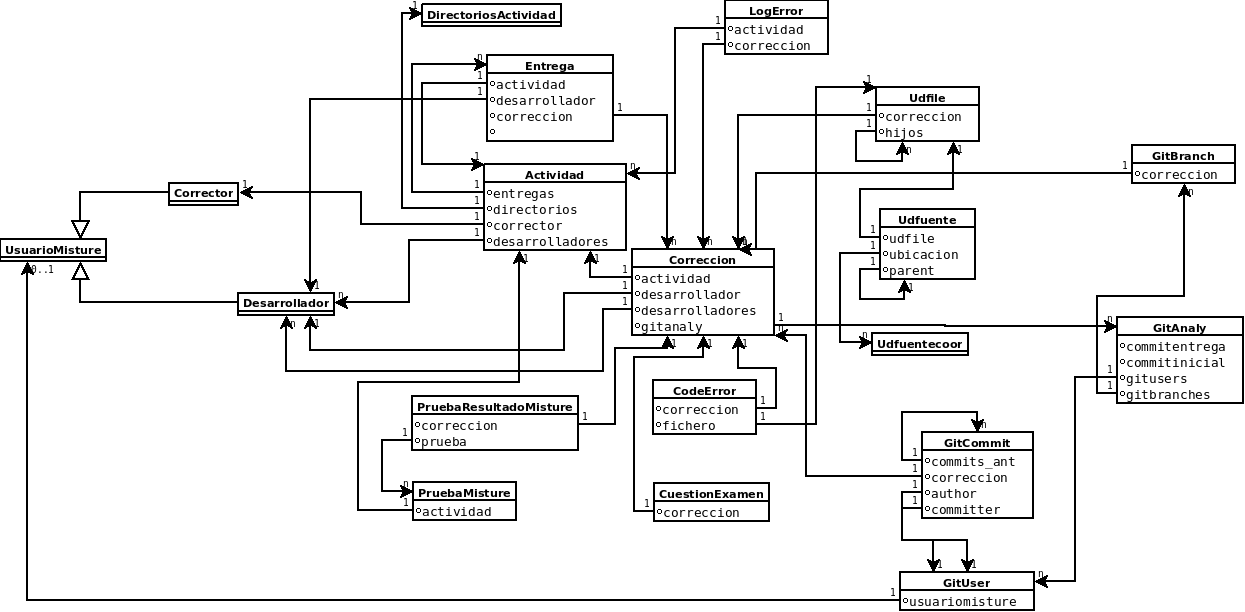
\includegraphics[width=16cm]{img/Diagram4_bbdd}
   \caption{Representación de BBDD incluida en Misture}
   \label{figura:bbdd}
\end{figure}

\vspace{3cm}



\begin{description}
\item \textbf{LogError} es la clase del documento donde se vuelcan los errores controlados de la ejecución de Misture.
\begin{itemize}
\item descripcion
\item accion
\item traza
\item fecha
\item actividad: referencia a \textbf{Actividad}
\item correccion: referencia a \textbf{Correccion}
\end{itemize}
\item \textbf{UsuarioMisture} representa a un usuario del sistema Misture.
\begin{itemize}
\item login
\item email
\item rol
\item date
\end{itemize}
\item \textbf{Corrector} es la clase heredera de \textbf{UsuarioMisture} que modela las particularidades del usuario corrector.
\begin{itemize}
\item actividades: referencia a \textbf{Actividad}
\item rol
\item superrol
\end{itemize}
\item \textbf{Desarrollador} es la subclasde de \textbf{UsuarioMisture} que representa al desarrollador.
\begin{itemize}
\item emails
\item rol
\end{itemize}
\item \textbf{}

\item \textbf{DirectoriosActividad} representan las rutas particulares donde se ubicarían los ficheros de la actividad a corregir.
\begin{itemize}
\item pbase
\item pentrega
\item presultados
\item perrores
\item ptest
\item ppruebas
\end{itemize}
\item \textbf{Actividad} es la clase que representa una actividad, con sus datos básicos para ser corregida.
\begin{itemize}
\item descripcion
\item corrector: referencia a \textbf{Corrector}
\item desarrolladores: referencia a \textbf{Desarrollador}
\item entregas: documento Entrega
\item directorios: documento \textbf{DirectoriosActividad}
\item ficheros\_entrega
\end{itemize}
\item \textbf{Correccion} es la clase que representa a la ejecución de una corrección de una entrega de un alumno.
\begin{itemize}
\item fecha
\item actividad: referencia a \textbf{Actividad}
\item desarrollador: referencia a \textbf{Desarrollador}
\item desarrolladores: referencia a \textbf{Desarrollador}
\item gitanaly: documento \textbf{GitAnaly}
\end{itemize}
\item \textbf{Entrega} es la clase que modela los elementos necesarios para emprender la corrección de la actividad de un alumno particular.
\begin{itemize}
\item actividad: referencia a \textbf{Actividad}
\item desarrollador: referencia a \textbf{Desarrollador}
\item modo
\item ubicacion
\item correccion: referencia al documento corrección.
\end{itemize}
\item \textbf{Udfile} representa a un fichero o directorio de una entrega.
\begin{itemize}
\item correccion: referencia a \textbf{Correccion}
\item pathrel
\item nombre
\item tipo
\item hijos: referencia a \textbf{Udfile}
\item lenguaje
\item sloc
\end{itemize}
\item \textbf{Udfuente} representa a un elemento de código dentro de un fichero fuente.
\begin{itemize}
\item udfile: referencia a Udfile
\item parent: referencia a Udfuente
\item nombre
\item ubicacion: documento Udfuentecoor
\item snippet
\end{itemize}
\item \textbf{Udfuentecoor} es la clase que modela la ubicación del elemento de código dentro de una fuente.
\begin{itemize}
\item filaini
\item filafin
\item col
\item pos
\end{itemize}

\item \textbf{}
\item \textbf{CodeError}: modela un error de estilo
\begin{itemize}
\item correccion: referencia a \textbf{Correccion}
\item fichero
\item fila
\item columna
\item tipo
\item codigo
\item descripcion
\end{itemize}
\item \textbf{GitUser}: usuario \textit{committer} o \textit{author} de Git.
\begin{itemize}
\item  name
\item email
\end{itemize}
\item \textbf{GitBranch}: datos de una rama de un repositorio Git de una corrección concreta.
\begin{itemize}
\item correccion: referencia a \textbf{Correccion}
\item nombre
\item nombre\_remote
\item targetid
\end{itemize}
\item \textbf{GitCommit}: representa un commit
\begin{itemize}
\item correccion: referencia a \textbf{Correccion}
\item idhex
\item orden
\item author: referencia a \textbf{GitUser}
\item committer: referencia a \textbf{GitUser}
\item time
\item offset
\item mensaje
\item palabrasclave
\item commits\_ant: referencia a \textbf{GitCommit}
\item ficheros
\end{itemize}
\item \textbf{GitAnaly} es la clase que contienen los datos de analisis de un repositorio Git.
\begin{itemize}
\item commitentrega: referencia a \textbf{GitCommit}
\item commitinicial: referencia a \textbf{GitCommit}
\item numcommits
\item palabras
\item intervalos
\item gitusers: referencia a \textbf{GitUser}
\item gitbranches: referencia a \textbf{GitBranch}
\end{itemize}
\item \textbf{PruebaMisture} representa la definición de una prueba de caja negra.
\begin{itemize}
\item actividad: referencia a \textbf{Actividad}.
\item titulo
\item descripcion
\item comando
\item salida
\end{itemize}
\item \textbf{PruebaResultadoMisture} representa el resultado de una ejecución de prueba sobre una corrección de una entrega particular.
\begin{itemize}
\item correccion: referencia a \textbf{Corrección}.
\item prueba: referencia a \textbf{PruebaMisture}
\item tipo\_salida
\item path\_salida
\item espruebavalida
\end{itemize}
\item \textbf{CuestionExamen} representa las preguntas del examen
\begin{itemize}
\item correccion: referencia a \textbf{Corrección}
\item tipo\_pregunta
\item contenido\_pregunta
\item tipo\_respuesta
\item opciones\_respuesta
\item opciones\_validas
\item respondida
\item respuesta
\item fecha\_respuesta
\end{itemize}
\end{description}
\cleardoublepage
\chapter{Resultados}
\label{chap:resultados}

Con la aplicación del proyecto Misture, pretendíamos, entre otros items a cumplir:\\


\begin{itemize}
\item Establecer un proyecto Python, que recoja las funciones básicas, detectadas en las muestras de las actividades entregables de las asignaturas de programación de aplicaciones y servicios web y multimedia en redes, adaptada a las pequeñas prácticas de los alumnos.

\item Automatizar la funcionalidad básica detectada, minimizando la cantidad de pasos o funcionalidades semiautomáticas o manuales llevadas a cabo por el profesor en las experiencias piloto.

\item Permitir cierta tolerancia en la automatización a errores por parte de los alumnos en los códigos o en los ficheros entregables. 

\item Disminuir el tiempo dedicado por el docente en el desarrollo o adaptación del código para la corrección de nuevas actividades, su ejecución, y la recogida de resultados y reporte de los puntos críticos a revisar.

\item Mejorar generación, riqueza, y comunicación del \textit{reporting} de los resultados de los diferentes análisis y correcciones que se ejecutan sobre los repositorios.

\item Mejorar la recogida de información extraída en las correcciones, de forma persistente y debidamente relacionada en sistemas de BBDD, permitiendo nuevos análisis posteriores, y ahorrando tiempo y re-ejecuciones en caso de errores que requieran alguna intervención manual por parte del profesor.

\item Interrelacionar nuestro sistema con una interfaz web, en una primera aproximación para la realización de exámenes de verificación de autoría y conocimiento del código del alumno.
\end{itemize}

De este compendio de deseos que inicialmente esperábamos cumplir, en el estadio en el que el proyecto Misture ha sido entregado, hemos llegado a los siguientes resultados.\


En cuanto a establecer un diseño que recoja la funcionalidad básica detectada en las experiencias piloto, podemos estimar que se ha podido realizar, con el diseño descrito en el apartado precedente. Asimismo, hemos construido una pequeña arquitectura, que en gran medida puede ser ampliada con nuevas funcionalidades y mejoras a partir de la propia estructura del proyecto y las BBDD propuestas.


Con respecto a los hitos de automatización, en algunas tareas concretas como el \textit{reporting} y comunicación de los resultados, que requerían mayor intervención manual, ha sido posible introducir una mayor ganancia en tiempo y en reducción de las intervenciones manuales por parte del profesor.


Sin embargo, en otras comprobaciones, como la comprobación de los ficheros entregados, el estilo y errores de los códigos fuentes, pruebas, etc. La ganancia principal, más que en tiempo, se produce en el hecho de disponer de los datos de los análisis almacenados sistemáticamente con una mayor riqueza y relacionados en un medio persistente -BBDD-.


En cambio, el permitir tolerancia en los procesos automáticos frente a pequeños errores de los alumnos ha sido uno de los hitos más complicados de cumplir.


En esa dirección se ha introducido alguna pequeña mejora, como la corrección con ayuda del algoritmo de Levenshtein de casos muy simples de equivocación de los nombres de los ficheros esperados, cuando se indica una lista obligatoria de ellos. Sin embargo, no ha sido posible encontrar soluciones abordables en el ámbito de este proyecto y en un plazo razonable para automatizar la rectificación de otros pequeños despistes que tienen los alumnos en sus entregas.


Por ejemplo, en casos en los que no se define estrictamente en el enunciado de la actividad propuesta, o el alumno comete errores, sobre la forma de usar o leer los parámetros de los \textit{scripts}. En este caso concreto esto puede dificultar tareas como la ejecución de pruebas de caja negra, y exigen al tutor pasar a operar manualmente, buscar y rectificar el problema, y realizar re-ejecuciones. También no poder evaluar por completo al alumno.


En general, podemos decir que con respecto a las experiencias piloto se ha mejorado en varios aspectos las tareas de corrección automática. También que con Misture se sienta una posible base sobre la que ampliar y mejorar funcionalidades y el reporte de información extraída y sus posibilidades de análisis.

Sin embargo, nos hemos encontrado con que no es tan fácil de alcanzar un grado elevado de generalización para abarcar escenarios de corrección menos específicos. Tampoco lo es alcanzar la automatización plena y desatendida de la herramienta, al menos en los procesos que hay entre la configuración de Misture y la  lectura de informes y reporte.

Por ejemplo, una ejecución de código de caja negra es difícil de adecuar para probar una práctica desarrollada en un \textit{framework} de aplicaciones web como Django, empleada por los alumnos en asignaturas de cursos más avanzados.

Por tanto, no hemos podido abarcar todas las automatizaciones que nos hubiera gustado.



\cleardoublepage
\chapter{Conclusiones}
\label{chap:conclusiones}

\section{LECCIONES APRENDIDAS}

Una de las principales lecciones aprendidas, consiste en entender la complejidad que resulta del diseño de herramientas que permitan la automatización de tareas.\\


La posibilidad de generar estos automatismos en casos lo más generalizables posibles debe estar muy bien estudiada en sus elementos o circunstancias para evitar encontrarse ante un caso complicado de manejar y de controlar en sus condiciones más probables.\\


Sino, o no es una tarea netamente automatizable, o debe ser considerada inclusive en subtareas más manejables y cuyos elementos característicos sean lo más homogéneos entre sí.\\


También puedo considerar que he aprendido algo mejor a evaluar mejor que proyectos o APIs debo elegir, y adquirido la noción de lo complejo que puede llegar a ser mantener en el tiempo pequeños proyectos de código abierto por parte de pequeños grupos de desarrolladores, a menudo de forma altruista en su tiempo libre.\\


El mayor ejemplo de esto que digo es el cambio que tuve que realizar del ODM mongoengine por pymodm, el primero bastante potente y con bastante historial detrás y que potencialmente podía facilitarme mucho una integración con Django.\\


Sin embargo, con el paso del tiempo y al utilizar más funcionalidades de este ODM y algunos fallos heredados de diseño de este, me empezó a generar diversos problemas y comportamientos inesperados para los que no encontraba solución, teniendo que cambiar y llevándome a sufrir una pérdida de tiempo considerable.\\


No obstante, otra opción es elegir uno de estos proyectos que a uno le resulte atractivo y sus colaboradores estén abiertos a colaboraciones, y colaborar con ellos.\\


Otra importante lección aprendida por parte mía, es quizás reconocer mi exceso de perfeccionismo en la realización de este tipo de tareas, en ocasiones por encima de la capacidad técnica que pueda tener en el momento dado, o la disponibilidad de tiempo o recursos para llevar a cabo su ejecución.\\


En muchas ocasiones, no palpar adecuadamente estos límites junto al ansia perfeccionista, me ha llevado a callejones sin salida, códigos complejos que he tenido que desechar, y derivas de tiempo.\\


No obstante, por otra parte, esa característica propia de mí, aplicada al mundillo profesional, me ha llevado a ser muy bien valorado como analista en varios de los proyectos en los que he trabajado. Sin embargo, la cantidad de estrés que en ocasiones genera esto, es excesivo.\\

\newpage
\section{CONOCIMIENTOS APLICADOS}

De una u otra forma, en la consecución de este proyecto, se han aplicado conocimientos adquiridos a lo largo de mi etapa universitaria cursando Ingeniería de Telecomunicación e Ingeniería Técnica en Informática de Sistemas.\\


Por una parte, hubo que recordar o aplicar conocimientos de la propia asignatura IARO, ya que alguna de las muestras de actividades empleadas para probar las funcionalidades correspondía a prácticas de contenido semejante a IARO.\\


Asimismo, nos aprovechamos del conocimiento adquirido en BBDD en las asignaturas de dicha temática. También de su uso en un framework como Django, cuya destreza adquirimos en materias como Sistemas y Aplicaciones Telemáticas.\\


También nos han sido útiles los conocimientos de otras materias como Ingeniería del Software y de Programación Orientada a Objetos.\\


No obstante, una vez afanados en encontrar relaciones, podríamos encontrarlas en todas las materias asociadas a la programación, BBDD, al desarrollo de software o a sistemas y aplicaciones web o de multimedia.\\

\newpage
\section{CONOCIMIENTOS ADQUIRIDOS}


Durante la investigación y desarrollo de Misture, he entrado en contacto con un buen número de conceptos, utilidades y tecnologías, algunas de las cuáles incluso excedían con creces la capacidad y tiempo que deben otorgarse a un Proyecto de Fin de Carrera y no he llegado a aplicar en el proyecto y por tanto mencionar aquí.\\


Entre aquellos conocimientos adquiridos y practicados se encuentran:\\


\begin{itemize}
\item El DBMS MongoDB. Además de los conceptos relativos a bases de datos NO-SQL o no relacionales.\\

\item Conocimientos sobre la herramienta Git y el manejo de repositorios distribuidos. Además del uso de los servicios Github y Gitlab.\\

\item Aunque Python ya era conocido para mí, se puede decir que también he aprendido acerca de Python 3, sus diferencias con respecto la versión 2, y las características nuevas que trae.\\

\item También se han adquirido conocimientos del uso y funcionamiento de diferentes herramientas de análisis estático, dinámico y de estilo del código, especialmente de aquellas orientadas al lenguaje Python: pep8, pylint, pymetrics, flake8, pyflakes, etc.

\end{itemize}

\newpage
\section{MEJORAS O TRABAJOS FUTUROS}


En este subapartado, se describen las posibles mejoras o líneas futuras que permitan un mayor desarrollo del proyecto obteniendo mejoras en el mismo.\\


Dado que personalmente observé y he observado en el tiempo una gran cantidad de opciones donde poder profundizar, pero que por complejidad o falta de tiempo no ha sido posible efectuar. Voy a detallar algunas funcionalidades o mejoras posibles que se pueden aplicar al proyecto propuesto:\\


\begin{itemize}
\item Ampliar el uso de la interfaz web como cliente integral para la fase inicial de configuración de la corrección de una actividad.\\

\item Ampliar las funcionalidades para hacer posible análisis entre de las diferentes actividades que con el tiempo se hayan corregido y pasen a formar parte de nuestro propio repositorio de correcciones.\\

\item Emplear las capacidades de módulos o librerías como ast o astor para posibilitar funcionalidades más potentes en los análisis de código fuente y su estructura, o para realizar pequeñas correcciones asistidas del código fuente sobre pequeños errores frecuentes de los alumnos que pueden dificultar la ejecución de tareas como las pruebas de ejecución.\\

\item Añadir nuevas formas de comunicación a la utilidad. Por ejemplo, añadir comunicación vía redes sociales tales como Twitter, Facebook o LinkedIn.\\

\item Integrar capacidades propias para detección de plagio.\\

\item Otra posibilidad a explorar, debido a la existencia de \textit{scripts} cliente y de librerías para la visualización y análisis de los resultados del análisis, es integrar la funcionalidad de MOSS en el propio Misture.\\
\end{itemize}


%
%%%%%%%%%%%%%%%%
% BIBLIOGRAFIA %
%%%%%%%%%%%%%%%%
\cleardoublepage

\begin{thebibliography}{25}
\bibliographystyle{alpha}

\bibitem{papers} Gregorio Robles y Jesús M. González-Barahona (2013). Mining student repositories to gain learning analytics

\bibitem{papers2} Robles, G., González-Barahona J. M., Izquierdo-Cortazar, D. y Herraiz, I. (2009). Tools for the Study of the Usual Data Sources found in Libre Software Projects.

\bibitem{msr} Web de las conferencias de MSR:   \\
{\footnotesize
\url{http://2017.msrconf.org/}} 

\bibitem{gitbook}Pro Git book. Scott Chacon and Ben Straub.   \\
{\footnotesize
\url{https://git-scm.com/book/es/v1}} 

\bibitem{pep8} Guía de estilo de Python PEP8.   \\
{\footnotesize
\url{https://www.python.org/dev/peps/pep-0008/}} 

\bibitem{analisis}Análisis estático de código.   \\
{\footnotesize
\url{http://raulexposito.com/documentos/analisis-estatico-codigo/}} 

\bibitem{p2}Referencia y librerías estándar de Python 2.   \\
{\footnotesize
\url{https://docs.python.org/2/}} 

\bibitem{p3}Referencia y librerías estándar de Python 3   \\
{\footnotesize
\url{https://docs.python.org/3/}} 

\bibitem{mongo}Documentación de MongoDB   \\
{\footnotesize
\url{https://docs.mongodb.com/manual/}} 

\bibitem{diferencia}Diferencias entre SQL y MongoDB   \\
{\footnotesize
\url{https://docs.mongodb.com/manual/reference/sql-comparison/}} 

\bibitem{pymongo}Documentación de la librería Pymongo   \\
{\footnotesize
\url{https://api.mongodb.com/python/current/}} 

\bibitem{pymod}Documentación de la librería PyMODM   \\
{\footnotesize
\url{https://github.com/mongodb/pymodm}} 

\bibitem{pygit2}Documentación de Pygit2   \\
{\footnotesize
\url{http://www.pygit2.org/}} 

\bibitem{flake8}Documentación de Flake8   \\
{\footnotesize
\url{https://flake8.readthedocs.io/en/latest/index.html}\\ \url{https://gitlab.com/pycqa/flake8}} 

\bibitem{pypep8}Documentación de la utilidad Pep8 -Pycodestyle-.  \\
{\footnotesize
\url{http://pep8.readthedocs.io/en/release-1.7.x/}\\
\url{https://github.com/PyCQA/pycodestyle}} 

\bibitem{pylint}Documentación de Pylint   \\
{\footnotesize
\url{https://pylint.readthedocs.io/en/latest/}} 

\bibitem{astor}Documentación de Astor.   \\
{\footnotesize
\url{https://github.com/berkerpeksag/astor}} 

\bibitem{pycharm}Web del IDE PyCharm   \\
{\footnotesize
\url{https://www.jetbrains.com/pycharm/}} 

\bibitem{robomongo}Web de la aplicación Robomongo.   \\
{\footnotesize
\url{https://robomongo.org/}}

\end{thebibliography}

\cleardoublepage
\appendix
\chapter{Instalación y Uso}
\label{app:instalacion}


Con el sistema Misture propuesto, si se desea efectuar una corrección con una parte o la totalidad de las funcionalidades básicas ya implementadas, sería necesario:\\

\begin{enumerate}
\item El directorio del profesor donde deposita los ficheros auxiliares a la corrección, tales como:\\

\begin{itemize}
\item Fichero con el listado de logines únicos de alumnos, emails, y ruta o url del repositorio individual. En este caso obligatorio.\\

\item Fichero con las preguntas estáticas de la prueba o examen que se mezclaran con las generadas de autoría.\\

\item Ficheros auxiliares para la ejecución de pruebas sobre el código: códigos de un servidor o cliente de prueba para lanzarlo contra el del alumno, xmls de configuración, ficheros de entrada sobre el que lanzar una prueba, etc.\\
\end{itemize}

\item Una copia del \textit{script} principal, que lee las configuraciones e invoca los diferentes submódulos de corrección.\\

\item Se utiliza a modo de plantilla, teniendo que ajustar la configuración y código del \textit{script}.\\

\item Estos ajustes a los módulos que realmente se van a utilizar entre aquellos que son opcionales, que llamadas se van a ejecutar en las pruebas y que resultado u listado de resultados válidos se pueden esperar.\\

\item Asimismo, se pueden ajustar otras constantes como el listado de errores o tipo de errores de pep8, pylint o hackings ignorar en un análisis de estilo y código.\\

\item También, en caso de activar la comprobación de xml o pdml, se indicarían cuáles comprobaciones, entre las implementadas, se deberían realizar, como la cuenta de trazas de determinado tipo en la captura Wireshark, la presencia de cierto atributo o valor en una etiqueta concreta, etc.\\
\end{enumerate}

\cleardoublepage

\chapter{Requisitos}
\label{app:req}

Para la ejecución del código de Misture.\\

En cuanto a librerías Python, si no se indica lo contrario, su instalación se aconseja realizar el gestor de paquetes Python Pip para instalar los paquetes necesarios en la versión 3 de Python, de la siguiente manera.\\


\begin{center}
\begin{verbatim}
pip3 install <nombre_paquete>
\end{verbatim}
\end{center}


Dada la cantidad de paquetes y dependencias manejados, se detallarán las dependencias principales, siendo instaladas todas las dependencias en las versiones disponibles o las requeridas por el propio paquete.\\


Además, por la misma razón, es una buena práctica configurar un ``Virtual Environment'' de Python específico para la configuración de todo el entorno necesario y la ejecución de este proyecto.\\


Una vez aclarado todo esto, definimos los principales requisitos:\\

\begin{itemize}
\item Interprete de Python: durante el desarrollo, se ha empleado principalmente el interprete de la versión 3.4, aconsejándose la instalación de la versión 3.4 o superior.\\

\item Asimismo, se dispuso de un interprete de la versión 2, en concreto de la versión 2.7, para el testing sobre códigos de Python 2. Aconsejándose, en caso de la corrección de prácticas en esa versión de Python, de un virtualenv con la versión más reciente utilizada por los alumnos.\\

\item Sistema gestor de bases de datos MongoDB: se ha empleado la versión 3.2.13.\\

\item La librería ODM ``pymodm'' de python: se aconseja usar la versión 0.4.0 o superior, teniendo en cuenta en la documentación de esta librería, se indica que está testeado para la versión de MongoDB que se tiene instalada.\\

\item Sistema de control de versiones Git: se recomienda tener instalada la versión 2 de este herramienta, ya que esta documentado y asimismo hemos detectado en diferentes pruebas con la librería que algunos de los comandos y opciones de Git han modificado su comportamiento, sus opciones por defecto, o el formato de su salida, afectando por tanto al comportamiento de pygit2.\\

\item Librería pygit2. El sistema Misture está probado con la versión 0.25.0\\

\item Librería Python de la herramienta flake8: se ha empleado la versión reciente 3.3.0.
\end{itemize}




\end{document}
